\documentclass[11pt]{article}
\usepackage[a4paper,margin=21mm,headheight=15pt]{geometry}
\usepackage{amsmath,amssymb,graphicx,booktabs,array,xcolor,fancyhdr,enumitem,hyperref}
\usepackage{fontspec}
\setmainfont{Times New Roman}
\setsansfont{Times New Roman}
\setmonofont{Consolas}[Scale=MatchLowercase]
\usepackage[italic]{mathastext}
\hypersetup{colorlinks=true,linkcolor=black,urlcolor=black}
\pagestyle{fancy}\fancyhf{}\lhead{FlowMLLab | Week 1.2}\rhead{Pressure--velocity coupling}\cfoot{\thepage}
\setlength{\emergencystretch}{3em}
\setlength{\parindent}{0pt}\setlength{\parskip}{7pt}
\setlist{nosep,leftmargin=*}
\newcommand{\topic}[2]{\section*{#1\quad #2}}
\begin{document}
\begin{center}
\vspace*{12mm}
{\Large FlowMLLab | Week 1.2}\\[12mm]
{\LARGE\bfseries Pressure--Velocity Coupling}\\[5mm]
{\Large SIMPLE, PISO and PIMPLE}\\[4mm]
{\large Finite-volume equations and the lid-driven cavity}\\[8mm]
Ehsan Roohi
\end{center}
\vspace{8mm}
\textbf{The central problem.} Momentum determines how fluid accelerates under pressure and viscous forces. Continuity constrains the resulting velocity. Pressure--velocity coupling obtains fields that satisfy both requirements on the same grid.

\textbf{Prerequisites.} Continuity and component momentum equations, finite differences, a linear system, and the Week 1 streamfunction--vorticity cavity example. Matrix notation is introduced after the scalar finite-volume equations.

\textbf{Learning outcomes.} Derive a cell pressure-correction equation; interpret predictor and corrected velocities; distinguish steady iteration, inner correction and outer correction; evaluate continuity, momentum defects, accuracy and computational work.

\begin{center}\begin{tabular}{ll}\toprule
Sections & Topics\\\midrule
1--4 & Conservation laws, staggered grid, momentum coefficients\\
5--8 & Pressure correction, conservation example and SIMPLE\\
9--11 & Backward Euler, PISO and a numerical correction example\\
12--15 & PIMPLE, nonlinear coefficient updates and convergence\\
16--21 & Recorded cavity comparisons and coupling study\\
22--23 & Notebook controls, exercises and references\\\bottomrule
\end{tabular}\end{center}
\textbf{Scope.} Two-dimensional, incompressible, laminar flow on a uniform staggered grid. The retained calculations compare $Re=100$, 400 and 1000. Higher-$Re$ spatial accuracy and transient accuracy require their own checks; convergence of a two-dimensional steady solver does not establish the physical stability of a three-dimensional flow.
\newpage
\topic{Reading map}{From a cell balance to a coupling algorithm}
\textbf{The physical question.} A guessed pressure field produces a velocity
from the momentum equations. Why might that velocity fail continuity?
The momentum solve uses the guessed pressure gradient; it has not yet imposed
zero net volume flux in every pressure cell. Pressure correction connects these
two requirements.

\begin{center}\begin{tabular}{p{.19\linewidth}p{.69\linewidth}}\toprule
Stage & Quantity to identify before moving on\\\midrule
1. Locate & Pressure at cell centers; horizontal and vertical velocities on their respective pressure-cell faces. Draw the separate momentum volume.\\
2. Balance & Integrate continuity over one pressure cell. East/north outflow is positive; west/south outflow is negative.\\
3. Predict & Use the current pressure in momentum to obtain tentative face velocities. Evaluate their cell imbalance.\\
4. Correct & Express a face-velocity increment using the pressure-correction difference across that face. Substitute into continuity to obtain the pressure equation.\\
5. Repeat & SIMPLE repeats the steady solve; PISO adds corrections within a time step; PIMPLE also updates momentum coefficients in an outer loop.\\\bottomrule
\end{tabular}\end{center}

\textbf{A small mass-balance check.} In a square pressure cell with $h=0.25$,
suppose the predicted face velocities are
$(u_e^*,u_w^*,v_n^*,v_s^*)=(0.12,0.08,0.01,0.03)$.
Their integrated outward volume flux per unit depth is
\[
Q_P^*=h(u_e^*-u_w^*+v_n^*-v_s^*)
=0.25(0.12-0.08+0.01-0.03)=0.005.
\]
The corresponding volume-normalized divergence is
$r_{c,P}^*=Q_P^*/h^2=0.08$. More fluid leaves this cell than enters it.
The correction must contribute $-0.005$ to the integrated outward flux.
It is determined together with neighboring cells, since they share faces.
Neither $Q_P^*$ nor $r_{c,P}^*$ is a pressure change.

\textbf{Companion reading.} The following freely accessible references provide
three complementary explanations:
\begin{itemize}
\item \href{https://doc.cfd.direct/notes/cfd-general-principles/pressure-velocity-coupling}{Section 5.10: pressure--velocity coupling}. Follow momentum rearrangement, face flux and substitution into continuity. The present lecture first expands those operations on a uniform staggered cell.
\item \href{https://www.openfoam.com/documentation/user-guide/6-solving/6.3-solution-and-algorithm-control}{OpenFOAM algorithm controls, section 6.3.3}. Compare the steady SIMPLE and transient PISO correction patterns.
\item \href{https://doc.cfd.direct/notes/cfd-general-principles/the-pimple-algorithm}{Section 5.21: PIMPLE}. Identify which coefficients change in the outer loop and why a steady pseudo-transient calculation is different from a time-accurate transient calculation.
\end{itemize}
These references also discuss collocated software implementations. Here the
grid is staggered; a software-specific face-interpolation rule should not be
substituted into this grid without deriving its corresponding balance.

\newpage
\topic{1}{Incompressible flow: conservation laws}
Horizontal velocity $u_d(x_d,y_d,t_d)$, vertical velocity $v_d(x_d,y_d,t_d)$ and pressure $p_d(x_d,y_d,t_d)$ are the unknown fields. Subscript $d$ denotes dimensional quantities. For a Newtonian fluid with constant density $\rho$ and constant kinematic viscosity $\nu$, with no body force, continuity is
\[
\frac{\partial u_d}{\partial x_d}+\frac{\partial v_d}{\partial y_d}=0.
\]
Conservation of horizontal and vertical momentum gives
\begin{align*}
\frac{\partial u_d}{\partial t_d}+u_d\frac{\partial u_d}{\partial x_d}+v_d\frac{\partial u_d}{\partial y_d}
&=-\frac{1}{\rho}\frac{\partial p_d}{\partial x_d}+\nu\left(\frac{\partial^2u_d}{\partial x_d^2}+\frac{\partial^2u_d}{\partial y_d^2}\right),\\
\frac{\partial v_d}{\partial t_d}+u_d\frac{\partial v_d}{\partial x_d}+v_d\frac{\partial v_d}{\partial y_d}
&=-\frac{1}{\rho}\frac{\partial p_d}{\partial y_d}+\nu\left(\frac{\partial^2v_d}{\partial x_d^2}+\frac{\partial^2v_d}{\partial y_d^2}\right).
\end{align*}
The left sides contain local and convective acceleration. Pressure gradients and viscous diffusion provide the right-side accelerations. These two equations and continuity form the incompressible Navier--Stokes system.

\textbf{Scales.} Let $L$ be cavity side length and $U$ the lid speed. Define $x=x_d/L$, $y=y_d/L$, $t=t_dU/L$, $u=u_d/U$, $v=v_d/U$, and $p=(p_d-p_{\rm ref})/(\rho U^2)$. Then $Re=UL/\nu$ and
\begin{align*}
\frac{\partial u}{\partial x}+\frac{\partial v}{\partial y}&=0,\\
\frac{\partial u}{\partial t}+u\frac{\partial u}{\partial x}+v\frac{\partial u}{\partial y}
&=-\frac{\partial p}{\partial x}+\frac{1}{Re}\left(\frac{\partial^2u}{\partial x^2}+\frac{\partial^2u}{\partial y^2}\right),\\
\frac{\partial v}{\partial t}+u\frac{\partial v}{\partial x}+v\frac{\partial v}{\partial y}
&=-\frac{\partial p}{\partial y}+\frac{1}{Re}\left(\frac{\partial^2v}{\partial x^2}+\frac{\partial^2v}{\partial y^2}\right).
\end{align*}
The following sections use these dimensionless quantities. At steady state the local time derivatives vanish, while convection, pressure and diffusion still balance.

\textbf{Cavity conditions.} The unit-square top lid has $u=1,v=0$; three stationary walls have $u=v=0$. Every wall is impermeable. The ideal moving-lid corners contain a velocity discontinuity, so pressure and vorticity extrema there require care. The introductory case is $Re=100$.
\newpage
\topic{2}{Staggered grid and cell mass balance}
Pressure is stored at the center of each square pressure cell. Horizontal velocity is stored on vertical faces and vertical velocity on horizontal faces. This is the staggered MAC arrangement. The spacing is $h=1/N$ for $N$ cells along one side.
\begin{center}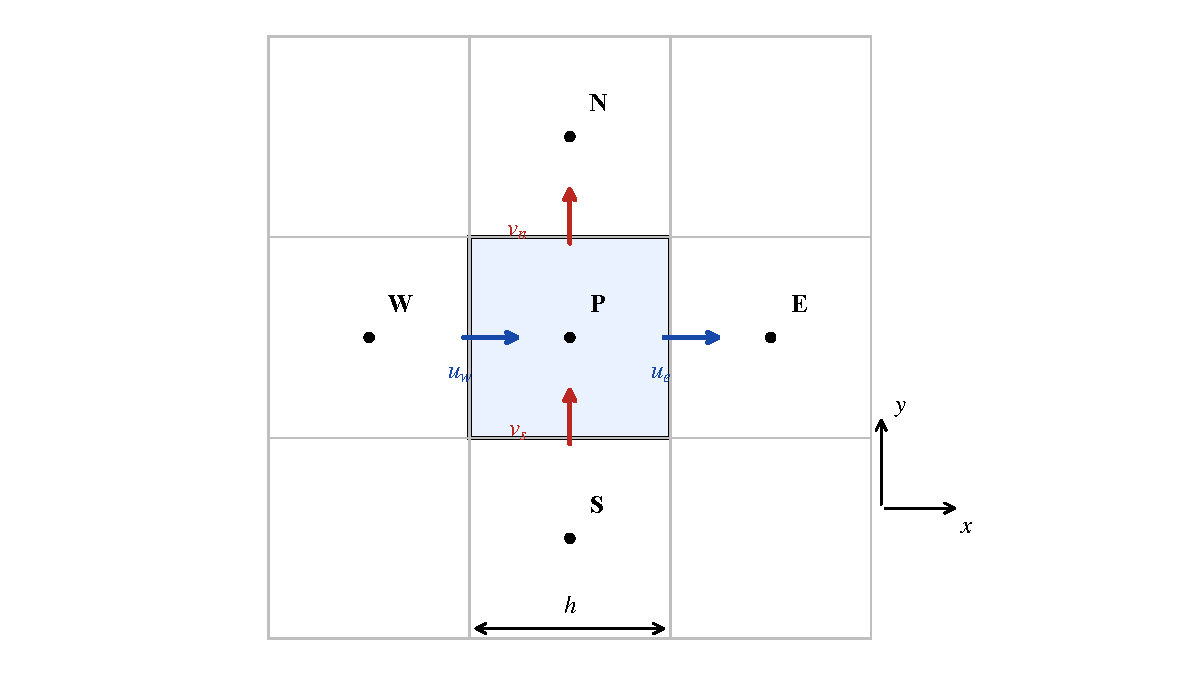
\includegraphics[width=.83\linewidth]{week01_2_assets/mac_grid.pdf}\end{center}
Capital $P,E,W,N,S$ label pressure-cell centers; lowercase $e,w,n,s$ label the four faces of cell $P$. All horizontal velocity components are positive rightward; all vertical components are positive upward. The outward normal at the west or south face points in the negative coordinate direction.

Integrating continuity over one cell and using the divergence theorem gives the net outward volume flux per unit depth:
\[
\int_{\partial V}\boldsymbol u\cdot\boldsymbol n\,\mathrm dS
=h u_e-h u_w+h v_n-h v_s=0.
\]
Dividing by the cell area $h^2$ gives the discrete divergence
\[
\boxed{\delta_P=\frac{u_e-u_w+v_n-v_s}{h}=0.}
\]
Density is constant, so zero volume imbalance also means zero mass imbalance. A shared face enters one cell with a plus sign and its neighbor with a minus sign. Summing all cell balances cancels internal fluxes; an impermeable boundary has zero total outward flux.

\textbf{Why pressure is needed.} A guessed pressure can satisfy the momentum equations for a tentative velocity yet leave $\delta_P\ne0$. The coupling algorithms adjust pressure gradients and face velocities together so that each cell satisfies continuity. Pressure is not prescribed independently throughout an incompressible cavity.
\newpage
\topic{3}{Finite-volume momentum at one velocity face}
The velocity $u_e$ lies between pressure centers $P$ and $E$. Its momentum control volume is centered on that velocity face. Integrating horizontal momentum over this control volume gives
\[
\frac{\mathrm d}{\mathrm dt}\int_{V_e}u\,\mathrm dV
+\int_{\partial V_e}u(\boldsymbol u\cdot\boldsymbol n)\,\mathrm dS
=-\int_{V_e}\frac{\partial p}{\partial x}\,\mathrm dV
+\frac{1}{Re}\int_{\partial V_e}\nabla u\cdot\boldsymbol n\,\mathrm dS.
\]
On the uniform interior grid, the volume-normalized pressure term is $-(p_E-p_P)/h$. Central interpolation approximates transported velocity at a momentum-volume face by the average of adjacent velocity samples. Central differences approximate its normal gradient.

\textbf{One interior row.} Denote the momentum control volume's neighboring horizontal velocities by $u_{\rm E},u_{\rm W},u_{\rm N},u_{\rm S}$; these are different samples of the same horizontal component. Its equation is
\[
\boxed{a_eu_e=a_{\rm E}u_{\rm E}+a_{\rm W}u_{\rm W}
+a_{\rm N}u_{\rm N}+a_{\rm S}u_{\rm S}+b_e-\frac{p_E-p_P}{h}.}
\]
Here $a_e$ is the center momentum coefficient, $a_{\rm NB}$ are neighbor coefficients, and $b_e$ contains known wall and time sources. All coefficients are normalized by control-volume area; no extra face area belongs in the pressure-gradient term.

Let $\beta=1/(Re\,h^2)$. Let $c_{\rm E},c_{\rm W}$ be the advecting horizontal velocities at the east/west boundaries of this momentum volume, and $c_{\rm N},c_{\rm S}$ the advecting vertical velocities at its north/south boundaries. The interior central scheme uses
\begin{align*}
a_{\rm E}&=\beta-\frac{c_{\rm E}}{2h},&a_{\rm W}&=\beta+\frac{c_{\rm W}}{2h},\\
a_{\rm N}&=\beta-\frac{c_{\rm N}}{2h},&a_{\rm S}&=\beta+\frac{c_{\rm S}}{2h},\\
a_e&=a_{\rm E}+a_{\rm W}+a_{\rm N}+a_{\rm S}
+\frac{c_{\rm E}-c_{\rm W}+c_{\rm N}-c_{\rm S}}{h}.
\end{align*}
For example, east-face convection contributes $c_{\rm E}(u_e+u_{\rm E})/(2h)$ on the left, and diffusion contributes $\beta(u_{\rm E}-u_e)$ on the right. Moving the convective neighbor term to the right leaves $(\beta-c_{\rm E}/(2h))u_{\rm E}$, which explains $a_{\rm E}$. Other faces follow from their outward-normal signs. Time and wall terms modify the diagonal and source. The vertical component has an analogous row.
\newpage
\topic{4}{Momentum coefficients and matrix notation}
For a face labeled $f$, collect the known source and neighbor contribution into
\[
H_f=b_f+\sum_{g\in\mathrm{NB}(f)}a_{fg}q_g,
\qquad d_f=\frac{1}{a_f}.
\]
The symbol $q_g$ means a velocity degree of freedom; it is not volume flux. The scalar momentum row becomes
\[
q_f=d_f\left[H_f-(Gp)_f\right],\qquad (Gp)_e=\frac{p_E-p_P}{h}.
\]
The vector $q$ collects all unknown interior horizontal and vertical face velocities. The scalar rows form two component linear systems, written together as
\[
Aq=b-Gp.
\]
The diagonal of $A$ contains the center coefficients $a_f$; its off-diagonal entries are $-a_{fg}$. With $R=A-\operatorname{diag}(a_f)$ and $d=\operatorname{diag}(1/a_f)$,
\[
H(q)=b-Rq,\qquad q=d\left[H(q)-Gp\right].
\]
Thus $H$ is computed from current neighbor velocities; it is not another fluid property. In this lesson $d$ is an inverse diagonal matrix, while $h$ is the mesh spacing.

\begin{center}\begin{tabular}{lll}\toprule
Symbol & Meaning & Location or role\\\midrule
$p$ & Pressure relative to a reference & Cell centers\\
$q$ & Collected velocity components & Interior faces\\
$A,b$ & Momentum matrix and source & Two component systems\\
$d$ & Inverse center coefficients & Face-wise diagonal\\
$R$ & Off-diagonal part of $A$ & Neighbor coupling\\
$H=b-Rq$ & Source plus neighbor terms & Recomputed from $q$\\
$D$ & Discrete divergence & Faces to cell balance\\
$G$ & Discrete pressure gradient & Centers to faces\\
$L=-DdG$ & Pressure operator & Cell-center system\\\bottomrule
\end{tabular}\end{center}
The notation abbreviates the scalar equations; it does not introduce additional physics. Each occurrence of $A,b,d$ refers to the current assembly, including any wall, transient or relaxation modifications.
\newpage
\topic{5}{Pressure correction from the momentum equations}
A star denotes a tentative velocity. A prime denotes a correction, not differentiation. Hold the momentum coefficients fixed while deriving one pressure correction. Given a pressure guess $p^k$, the predictor satisfies
\[
Aq^*=b-Gp^k.
\]
Write $q=q^*+q'$ and $p=p^k+p'$. Substituting these into the same momentum system and subtracting the predictor gives
\[
Aq'=-Gp'.
\]
At one horizontal face this is
\[
a_eu'_e=\sum_{g\in\mathrm{NB}(e)}a_{eg}q'_g-\frac{p'_E-p'_P}{h}.
\]
The exact correction couples neighboring velocity corrections. SIMPLE obtains a local correction by neglecting that neighbor-correction sum during this correction solve:
\[
\boxed{u'_e=-d_e\frac{p'_E-p'_P}{h}},\qquad d_e=1/a_e.
\]
Likewise,
\begin{align*}
u'_w&=-d_w\frac{p'_P-p'_W}{h},\\
v'_n&=-d_n\frac{p'_N-p'_P}{h},&
v'_s&=-d_s\frac{p'_P-p'_S}{h}.
\end{align*}
The corrected velocity must satisfy cell continuity. Substituting the four face corrections gives
\[
0=\delta_P^*+\frac{u'_e-u'_w+v'_n-v'_s}{h},
\qquad\delta_P^*=\frac{u_e^*-u_w^*+v_n^*-v_s^*}{h}.
\]
This equation determines pressure corrections from the predictor's cell imbalance. Neglecting neighbor corrections is an approximation to momentum coupling, not permission to violate continuity. Repeated coupling iterations are required to recover the target steady momentum solution.
\newpage
\topic{6}{The cell pressure equation and its boundary data}
For an interior cell, insert the four gradient expressions into corrected continuity and collect coefficients of pressure:
\begin{align*}
&\frac{d_e+d_w+d_n+d_s}{h^2}p'_P\\
&\quad-\frac{d_ep'_E+d_wp'_W+d_np'_N+d_sp'_S}{h^2}
=-\delta_P^*.
\end{align*}
The center coefficient is the sum of four face weights; each neighbor has a negative coefficient. The right side is the negative cell divergence of the tentative velocity. The same face weight must be shared by its two adjacent pressure cells.

\textbf{Matrix form.} Applying $D$ to $q=q^*-dGp'$ gives
\begin{align*}
0&=Dq^*-DdGp',\\
L&=-DdG,\\
Lp'&=-Dq^*.
\end{align*}
The positive-diagonal convention for $L$ explains the minus sign on the right. Once pressure is solved, the face correction $-dGp'$ cancels the computed cell imbalance, up to linear-solve error.

\textbf{Impermeable walls.} The normal wall velocity is prescribed and is not an unknown interior face velocity. Its normal correction is zero. A prescribed wall-normal face contributes zero correction weight, so that face coefficient is omitted from the boundary-cell pressure row. Pressure assembly therefore has no correction flux across the external wall. This is equivalent to the appropriate homogeneous normal pressure-correction condition for a predictor that already satisfies wall-normal velocity.

\textbf{Pressure reference.} Adding a constant to every cell pressure changes no pressure gradient: $G\boldsymbol 1=0$. Consequently $L\boldsymbol 1=0$ and the closed-cavity pressure system has one arbitrary constant. The implementation pins one pressure cell during the solve and removes the mean afterward. The reported zero-mean pressure is a gauge choice, not an extra boundary force.

Tangential no-slip is enforced in momentum through wall diffusion. On the staggered grid it is distinct from the zero normal correction used in the cell mass balance.
\newpage
\topic{7}{Two-cell pressure-correction example}
Consider two closed square cells with one shared vertical face. This is an algebraic conservation example, not a resolved cavity. Let $h=0.5$, tentative shared velocity $u^*=0.2$, and inverse momentum diagonal $d_e=0.1$. Positive shared velocity leaves cell 1 and enters cell 2. All external normal velocities are zero.
\[
\delta_1^*=\frac{0.2}{0.5}=0.4,\qquad
\delta_2^*=\frac{-0.2}{0.5}=-0.4.
\]
The shared pressure weight is $d_e/h^2=0.1/0.25=0.4$. Therefore
\[
0.4\begin{bmatrix}1&-1\\-1&1\end{bmatrix}
\begin{bmatrix}p'_1\\p'_2\end{bmatrix}
=\begin{bmatrix}-0.4\\0.4\end{bmatrix}.
\]
The first row gives $p'_1-p'_2=-1$. With zero mean, $p'_1+p'_2=0$, so $p'_1=-0.5$ and $p'_2=0.5$. The corrected face velocity is
\[
u=u^*-d_e\frac{p'_2-p'_1}{h}
=0.2-0.1\frac{0.5-(-0.5)}{0.5}=0.
\]
Both corrected divergences are zero. A common constant added to $p'_1$ and $p'_2$ leaves this calculation unchanged.

\textbf{Pressure relaxation and velocity correction.} If only $\alpha_p=0.3$ of the velocity correction were applied, the shared velocity would remain $0.2-0.3(0.2)=0.14$. The two mass defects would then be $+0.28$ and $-0.28$. Therefore the conservative velocity correction is applied fully, even when the pressure field used in the next momentum predictor is relaxed.

\textbf{Local and global conservation.} The initial global sum was already $0.4-0.4=0$, but each cell was imbalanced. A zero total boundary flux alone cannot certify local continuity.
\newpage
\topic{8}{SIMPLE: steady pressure--velocity coupling}
SIMPLE means Semi-Implicit Method for Pressure-Linked Equations. Its index $k$ counts steady coupling iterations, not physical time. Each iteration assembles convection from the latest velocity, solves a momentum predictor, then solves the pressure-correction equation.

\textbf{Momentum under-relaxation.} Let $a_f^0$ be the original center coefficient of the current unrelaxed assembly. For $0<\alpha_u\leq1$, the relaxed row uses
\[
a_f^{\rm rel}=\frac{a_f^0}{\alpha_u},\qquad
b_f^{\rm rel}=b_f+\left(\frac{1}{\alpha_u}-1\right)a_f^0q_f^k.
\]
The added source uses the original diagonal $a_f^0$. At a converged fixed point, $q_f^{k+1}=q_f^k$, the added diagonal and source contributions cancel. The target steady equation is unchanged. The pressure correction uses $d_f=1/a_f^{\rm rel}$.

\textbf{One steady iteration.}
\begin{align*}
A^{\rm rel}q^*&=b^{\rm rel}-Gp^k,\\
Lp'&=-Dq^*,\\
q^{k+1}&=q^*-dGp',\\
p^{k+1}&=p^k+\alpha_p p',\qquad 0<\alpha_p\leq1.
\end{align*}
Velocity is corrected fully; only the stored pressure update is damped by $\alpha_p$. After boundary conditions and the pressure gauge are applied, the next iteration rebuilds the momentum coefficients from the corrected velocity.

\textbf{Stopping criteria.} Momentum relaxation can make updates small before the original equations are satisfied. The implementation checks the unrelaxed nonlinear steady momentum defect and the cell divergence. Both must meet tolerance. In the retained baseline, $\alpha_u=0.7$ and $\alpha_p=0.3$.

\textbf{Role.} SIMPLE is a natural steady solver. It can also be used inside a transient nonlinear solve, but the current implementation's SIMPLE branch has no physical time step. Its iteration count cannot be compared directly with the physical-step counts of PISO or PIMPLE.
\newpage
\topic{9}{Physical time and backward-Euler momentum}
PISO and PIMPLE solve a transient momentum equation. Superscripts $n$ and $n+1$ denote physical time levels, separated by $\Delta t$. For one face velocity,
\[
\left.\frac{\partial q_f}{\partial t}\right|_{n+1}
\approx\frac{q_f^{n+1}-q_f^n}{\Delta t}.
\]
If the spatial momentum row has center coefficient $a_f^{\rm space}$ and source $b_f^{\rm space}$, backward Euler produces
\begin{align*}
\left(a_f^{\rm space}+\frac{1}{\Delta t}\right)q_f^{n+1}
&=\sum_g a_{fg}q_g^{n+1}+b_f^{\rm space}
+\frac{q_f^n}{\Delta t}-(Gp^{n+1})_f.
\end{align*}
Thus the transient assembly adds $1/\Delta t$ to the diagonal and the known old velocity $q_f^n/\Delta t$ to the source.

\textbf{Old-time velocity is fixed.} At the beginning of the physical step, store $q^n$. Every momentum assembly and every correction within that step uses the same old-time source. Replacing $q^n$ with an intermediate corrected velocity would change the discrete physical problem.

\textbf{Nonlinear coefficients.} Convective coefficients depend on advecting velocity. They must be evaluated from a known estimate to form a linear predictor system. Such coefficients are called frozen or lagged during that solve. A perfectly solved linear predictor can still differ from the fully implicit nonlinear step if its coefficients were evaluated at an outdated velocity.

\textbf{Three iteration levels.} A linear solver solves one matrix equation. A pressure corrector couples pressure and velocity for a frozen momentum matrix. An outer corrector rebuilds that matrix using the latest velocity. None of these is an additional physical time advance.

Backward Euler is first-order accurate in time. Extra correctors can reduce algebraic coupling error, but do not change its time-discretization order. A larger stable $\Delta t$ still requires a temporal-accuracy assessment.
\newpage
\topic{10}{PISO: pressure corrections for a frozen momentum matrix}
PISO means Pressure-Implicit with Splitting of Operators. At one physical step, assemble transient momentum once and solve
\[
Aq^*=b-Gp^{\rm guess}.
\]
This predictor uses the pressure available from the preceding step or initial state. Its momentum residual for that pressure can be small, while its cell divergence is nonzero.

Set $q^{(0)}=q^*$. The index $m$ counts inner corrections within this one physical step. The component matrices $A$, their source $b$, inverse diagonal $d$, off-diagonal part $R$, and pressure operator $L=-DdG$ remain fixed throughout the inner loop. Neighbor velocities do change, so each correction computes
\begin{align*}
H^{(m)}&=b-Rq^{(m)},\\
Lp^{(m+1)}&=-D\left(dH^{(m)}\right),\\
q^{(m+1)}&=d\left[H^{(m)}-Gp^{(m+1)}\right].
\end{align*}
The pressure equation follows by applying $D$ to the last line and imposing $Dq^{(m+1)}=0$. Unlike SIMPLE's $p'$, this implementation's $p^{(m+1)}$ is the full pressure field in the chosen gauge, rather than a pressure increment. It replaces the previous pressure; it is not added to it.

\textbf{Purpose of the next correction.} Reconstructed velocity changes the neighbor terms in $H$. Recomputing $H$ and solving pressure again improves the consistency of reconstructed velocity with the same frozen momentum equation. Repeating a linear pressure solve with an unchanged right-hand side is not an additional PISO correction.

After $N_i$ corrections, accept $q^{n+1}=q^{(N_i)}$ and $p^{n+1}=p^{(N_i)}$, then advance time once. The retained baseline has $N_i=2$. No momentum or pressure relaxation is applied by this transient branch.

The nonlinear convection coefficients remain those used for the initial predictor. That limitation motivates an outer coefficient-update loop.
\newpage
\topic{11}{PISO: a frozen-matrix numerical example}
This reduced two-velocity system illustrates coupling algebra; it is not a cavity grid. Let
\[
A=\begin{bmatrix}4&1\\1&3\end{bmatrix},\quad
b=\begin{bmatrix}2\\0\end{bmatrix},\quad
D=\begin{bmatrix}1&-1\end{bmatrix},\quad
G=\begin{bmatrix}-1\\1\end{bmatrix}.
\]
The scalar $p$ is one gauge-reduced pressure degree of freedom. Continuity is $Dq=q_1-q_2=0$. From $A$,
\[
d=\begin{bmatrix}1/4&0\\0&1/3\end{bmatrix},\quad
R=\begin{bmatrix}0&1\\1&0\end{bmatrix},\quad L=-DdG=7/12.
\]
Starting from $p^{\rm guess}=0$, the momentum predictor solves $Aq^*=b$:
\[
q^*=\begin{bmatrix}6/11\\-2/11\end{bmatrix},\qquad Dq^*=8/11.
\]
It satisfies momentum exactly but violates continuity. The first inner correction uses
\[
H^{(0)}=b-Rq^*=\begin{bmatrix}24/11\\-6/11\end{bmatrix},\qquad
dH^{(0)}=\begin{bmatrix}6/11\\-2/11\end{bmatrix}.
\]
Solve pressure and reconstruct velocity:
\begin{align*}
\frac{7}{12}p^{(1)}&=-D(dH^{(0)})=-\frac{8}{11},&p^{(1)}&=-\frac{96}{77},\\
q_1^{(1)}&=\frac14\left(\frac{24}{11}+p^{(1)}\right)=\frac{18}{77},&
q_2^{(1)}&=\frac13\left(-\frac{6}{11}-p^{(1)}\right)=\frac{18}{77}.
\end{align*}
The signs in these two velocity formulas follow from $G=(-1,1)^T$. Now $Dq^{(1)}=0$. Nevertheless, substituting these fields into the original frozen momentum equation gives
\[
r^{(1)}=Aq^{(1)}-b+Gp^{(1)}
=\begin{bmatrix}32/77\\-24/77\end{bmatrix}.
\]
Mass balance is exact, but momentum consistency still needs improvement.
\newpage
\topic{11 continued}{The second pressure correction}
The corrected neighbor velocities change $H$, even though $A$ and $L$ are unchanged:
\[
H^{(1)}=b-Rq^{(1)}=\begin{bmatrix}136/77\\-18/77\end{bmatrix},\qquad
dH^{(1)}=\begin{bmatrix}34/77\\-6/77\end{bmatrix}.
\]
The next pressure and velocity are
\begin{align*}
\frac{7}{12}p^{(2)}&=-\frac{40}{77},&p^{(2)}&=-\frac{480}{539},\\
q^{(2)}&=d\left[H^{(1)}-Gp^{(2)}\right]
=\begin{bmatrix}118/539\\118/539\end{bmatrix}.
\end{align*}
The pressure is replaced by $p^{(2)}$; adding $p^{(2)}$ to $p^{(1)}$ would be incorrect. Again continuity is exact. The remaining frozen-momentum defect is
\[
r^{(2)}=\begin{bmatrix}-8/539\\-8/539\end{bmatrix}.
\]
\begin{center}\begin{tabular}{lrr}\toprule
Stage & $|Dq|$ & $\|Aq-b+Gp\|_\infty$\\\midrule
Momentum predictor & $8/11$ & $0$\\
Inner correction 1 & $0$ & $32/77\approx0.41558$\\
Inner correction 2 & $0$ & $8/539\approx0.01484$\\\bottomrule
\end{tabular}\end{center}
The exact constrained solution is $q_1=q_2=2/9$ and $p=-8/9$. It follows by imposing $q_1=q_2=s$ in both original momentum rows: $5s-p=2$ and $4s+p=0$, hence $9s=2$.

The second correction reduces momentum inconsistency in this example while preserving mass balance. This is a demonstrated property of these specified matrices, not a guarantee of monotone convergence for every CFD system.

The right-hand side of the pressure equation changes from $-8/11$ to $-40/77$. The example therefore distinguishes another PISO correction from another iteration of an unchanged linear pressure solve.
\newpage
\topic{12}{PIMPLE: outer coefficient updates and inner corrections}
PIMPLE combines an outer momentum-update loop with PISO inner corrections. Physical time levels are $n,n+1$; $\ell$ labels outer updates and $m$ labels inner pressure corrections. The previous physical velocity $q^n$ is stored once.

At the start of outer pass $\ell$, assemble convection using the latest available corrected velocity $\widehat q^{(\ell)}$. This gives new matrices and sources
\[
A^{(\ell)}=A_{\rm space}(\widehat q^{(\ell)})+I/\Delta t,
\qquad b^{(\ell)}=b_{\rm wall}^{(\ell)}+q^n/\Delta t.
\]
Here $I$ is the identity matrix. The same $q^n$ appears in every outer pass. Wall contributions may depend on the current assembly, but the prescribed wall motion and old-time source belong to the same physical step.

The first outer pass starts from $q^n,p^n$. The symbol $\widehat p^{(\ell)}$ denotes the latest available pressure at the start of outer pass $\ell$. A new momentum predictor is solved using that pressure. Then inner corrections hold the current outer assembly fixed:
\begin{align*}
A^{(\ell)}q^{(\ell,0)}&=b^{(\ell)}-G\widehat p^{(\ell)},\\
H^{(\ell,m)}&=b^{(\ell)}-R^{(\ell)}q^{(\ell,m)},\\
L^{(\ell)}p^{(\ell,m+1)}&=-D\left(d^{(\ell)}H^{(\ell,m)}\right),\\
q^{(\ell,m+1)}&=d^{(\ell)}\left[H^{(\ell,m)}-Gp^{(\ell,m+1)}\right].
\end{align*}
The final corrected fields of one outer pass initialize the next. Rebuilding $A$ also rebuilds $d$, $R$ and $L$. Each inner solve computes the full pressure field in the chosen gauge, as in this PISO implementation.

\textbf{Two different purposes.} Inner corrections improve pressure--velocity consistency for the current matrix. Outer passes update the nonlinear coefficients that matrix represents. Neither loop advances physical time. Only after the final outer pass are the accepted fields assigned to time $n+1$.

With one outer pass, this code reduces to its PISO algorithm. Its PIMPLE branch does not apply SIMPLE's under-relaxation. Additional loops reduce certain algebraic errors at extra cost; they do not increase backward-Euler's formal time order.
\newpage
\topic{13}{PIMPLE: a nonlinear coefficient example}
Extend the preceding algebraic example by making its momentum coefficients depend on velocity:
\[
A(s)=\begin{bmatrix}4+s&1\\1&3+s\end{bmatrix},\qquad
s=(q_1+q_2)/2,\qquad b=\begin{bmatrix}2\\0\end{bmatrix}.
\]
Keep the same $D,G$ and initial $q=0,p=0$. At each outer pass, evaluate $s$ from its starting velocity, freeze $A(s)$, solve a new predictor, and perform two inner corrections. The source $b$ remains fixed. This toy coefficient law illustrates lagging; it is not a Navier--Stokes convection discretization.

At outer pass 1, $s=0$, so the two inner corrections are exactly the previous PISO example. They end at $q_1=q_2=0.2189239332$. The next outer pass uses
\[
A^{(2)}=\begin{bmatrix}4.2189239332&1\\1&3.2189239332\end{bmatrix},
\]
and recomputes $d,R,L$ before the new predictor and inner corrections.

\begin{center}\small\begin{tabular}{rrrrr}\toprule
Outer pass & Frozen $s$ & Final $q_1=q_2$ & Final $p$ & Nonlinear defect\\\midrule
1 & $0$ & $0.2189239332$ & $-0.8905380334$ & $3.30854\times10^{-2}$\\
2 & $0.2189239332$ & $0.2119026446$ & $-0.8940486777$ & $1.53537\times10^{-3}$\\
3 & $0.2119026446$ & $0.2122289655$ & $-0.8938855173$ & $7.14784\times10^{-5}$\\\bottomrule
\end{tabular}\end{center}
The reported defect evaluates the nonlinear equation using the final velocity:
\[
\left\|A\left((q_1+q_2)/2\right)q-b+Gp\right\|_\infty.
\]
It is different from the residual of the frozen predictor matrix. All final mass defects are below $10^{-15}$.

For the exact constrained solution set $q_1=q_2=s$ and add the two momentum rows:
\[
(9+2s)s=2,\qquad
s=\frac{\sqrt{97}-9}{4}=0.2122144504,\qquad p=s/2-1.
\]
The table shows the benefit of coefficient updates for this example. Actual cavity efficiency must be judged using its own measured equation defects, accuracy and solve costs.
\newpage
\topic{14}{Algorithm loops and computational work}
\begin{center}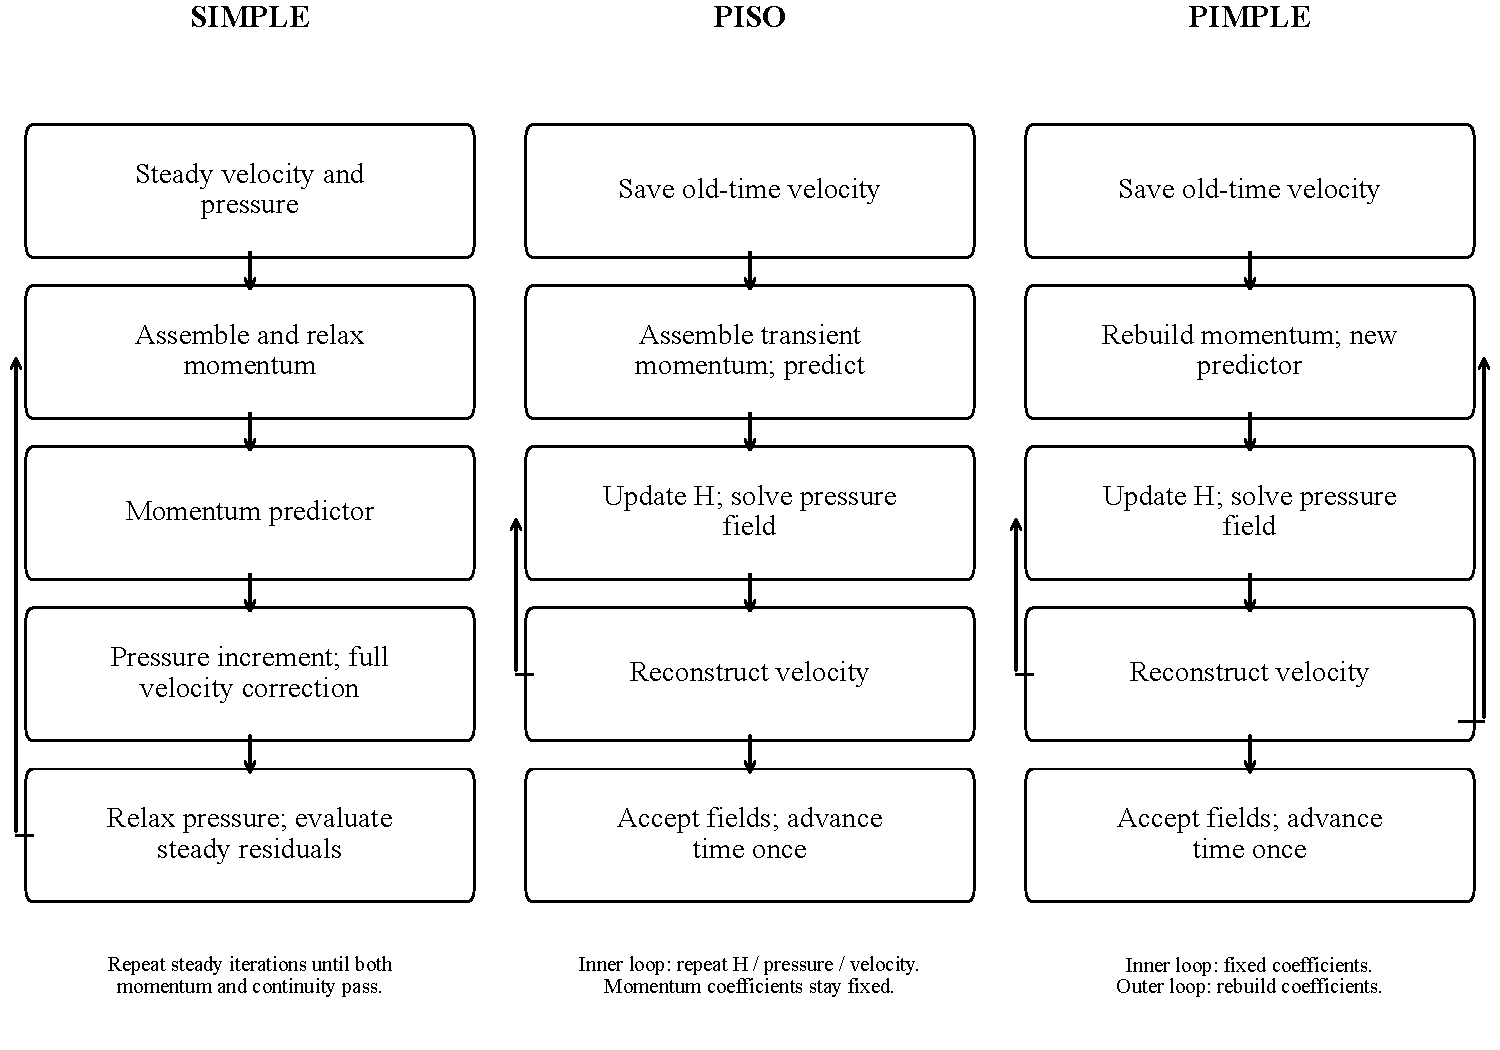
\includegraphics[width=.96\linewidth]{week01_2_assets/loop_map.pdf}\end{center}
The nested loops act on one target problem at the current physical step. The diagram distinguishes steady SIMPLE iterations from PISO and PIMPLE time integration.

Let $N_i$ be the number of pressure correctors and $N_o$ the number of outer correctors. Each predictor solves horizontal and vertical momentum separately.
\begin{center}\begin{tabular}{lrrr}\toprule
Work unit & SIMPLE iteration & PISO step & PIMPLE step\\\midrule
Momentum assemblies & $1$ & $1$ & $N_o$\\
Component momentum solves & $2$ & $2$ & $2N_o$\\
Pressure solves & $1$ & $N_i$ & $N_oN_i$\\
Physical time advances & $0$ & $1$ & $1$\\\bottomrule
\end{tabular}\end{center}
For three outer and two inner correctors, PIMPLE uses three assemblies, six component momentum solves and six pressure solves per physical step. A direct linear solver may factor a pressure matrix once and reuse it within an inner loop, while solving different right-hand sides.

An iteration count alone cannot compare these costs. The retained runs use fixed corrector counts, rather than an adaptive inner tolerance. A steady stopping test is applied outside these operations.
\newpage
\topic{15}{Convergence, accuracy and the meaning of a residual}
\textbf{Cell continuity.} The mass-balance diagnostic is $\max_P|\delta_P|$. It is evaluated from face velocities, not from an interpolated picture of cell-center velocity.

\textbf{Momentum defect.} For a steady target, the implementation rebuilds the unrelaxed spatial coefficients using final velocity and evaluates the original momentum equations. For a transient step, a nonlinear step defect includes the same fixed old-time source:
\[
r_{\rm step}=A_{\rm space}(q^{n+1})q^{n+1}-b_{\rm wall}
+\frac{q^{n+1}-q^n}{\Delta t}+Gp^{n+1}.
\]
Small mass defect alone does not make this vector small, as the PISO numerical example demonstrated.

\textbf{Accuracy.} Agreement with independent reference velocities and stability under spatial refinement address solution accuracy. Ghia centerline tables validate selected velocity profiles; they do not validate pressure. A converged coarse-grid calculation can still be inaccurate.

\textbf{Transient accuracy.} Corrector loops reduce algebraic errors inside a step. Temporal error is assessed separately by reducing $\Delta t$ and comparing at matched physical times. Steady cavity agreement alone does not validate startup or oscillatory flow.

\textbf{Streamfunction--vorticity comparison.} Week 1 advances vorticity and solves streamfunction. Its native update norm is different from the finite-volume momentum defect. Their convergence histories use separate axes; common velocity errors and wall-clock times provide cross-formulation comparisons. $N$ finite-volume cells correspond to $N+1$ finite-difference nodes at matching spacing $h=1/N$.

\textbf{Higher Reynolds numbers.} Stronger convection and thinner layers can require more cells and more work. More pressure corrections cannot recover spatial structures missing from the mesh. Refinement and higher-$Re$ runs can take substantially longer and need more memory; the supplied coarse cases are the starting point for laptop or Colab use.

\newpage
\topic{16}{Recorded cavity accuracy and runtime at $Re=100$}
\begin{center}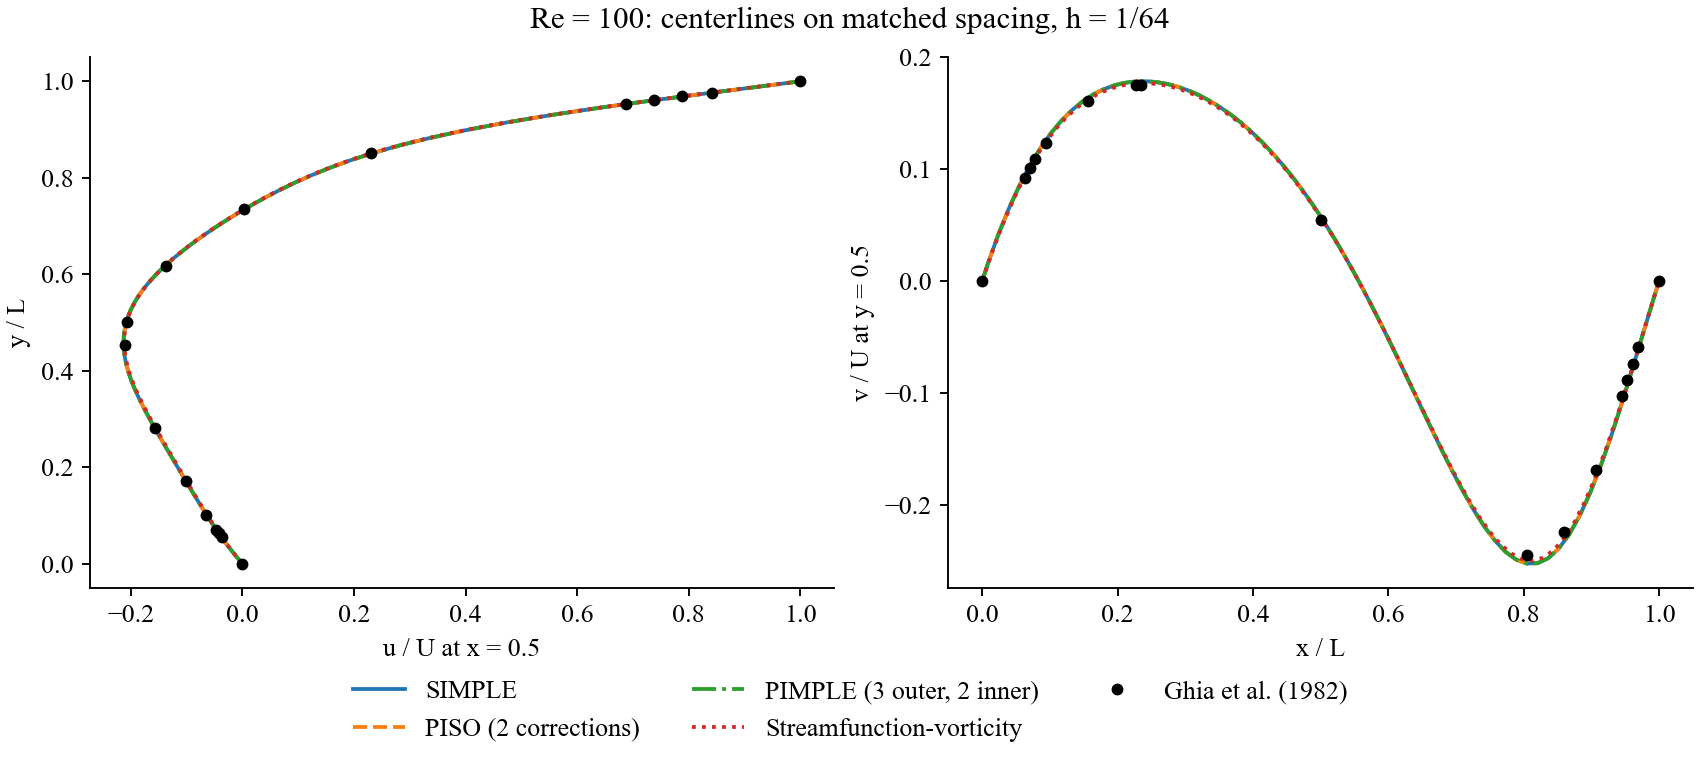
\includegraphics[width=.95\linewidth,height=64mm,keepaspectratio]{../../results/week01_2_pressure_velocity/figures/centerlines.png}\end{center}
The Ghia velocity markers are independent reference samples. The three finite-volume coupling methods use the same spatial equations. Their converged fields agree closely; differences from the finite-difference formulation also include spatial-discretization differences. The displayed 32/64 finite-volume cell counts correspond to 33/65 finite-difference nodes.
\begin{center}\small
\begin{tabular}{lrrr}\toprule
Formulation & Cells per side & Iterations / steps & Recorded seconds\\\midrule
SIMPLE & 32 & 480 & 5.074\\
PISO & 32 & 540 & 6.994\\
PIMPLE & 32 & 540 & 19.604\\
Streamfunction--vorticity & 32 & 19000 & 8.106\\
SIMPLE & 64 & 1870 & 137.987\\
PISO & 64 & 540 & 42.756\\
PIMPLE & 64 & 540 & 146.522\\
Streamfunction--vorticity & 64 & 19000 & 17.284\\
\bottomrule\end{tabular}\end{center}

The table includes all four formulations and reports recorded solver-call seconds. The finite-difference reference has its own stopping norm and recovers pressure afterward. These measurements depend on the host, implementation, mesh, relaxation and stopping targets; they do not establish a universal fastest method.

The finite-difference centerline errors decrease on refinement in this retained comparison. The finite-volume Ghia errors are not monotone between the two supplied grids. That behavior is retained rather than interpreted as proof of grid independence. More resolution and reference evidence are needed for an asymptotic accuracy claim.
\newpage
\topic{17}{Velocity structure and vorticity}
\begin{center}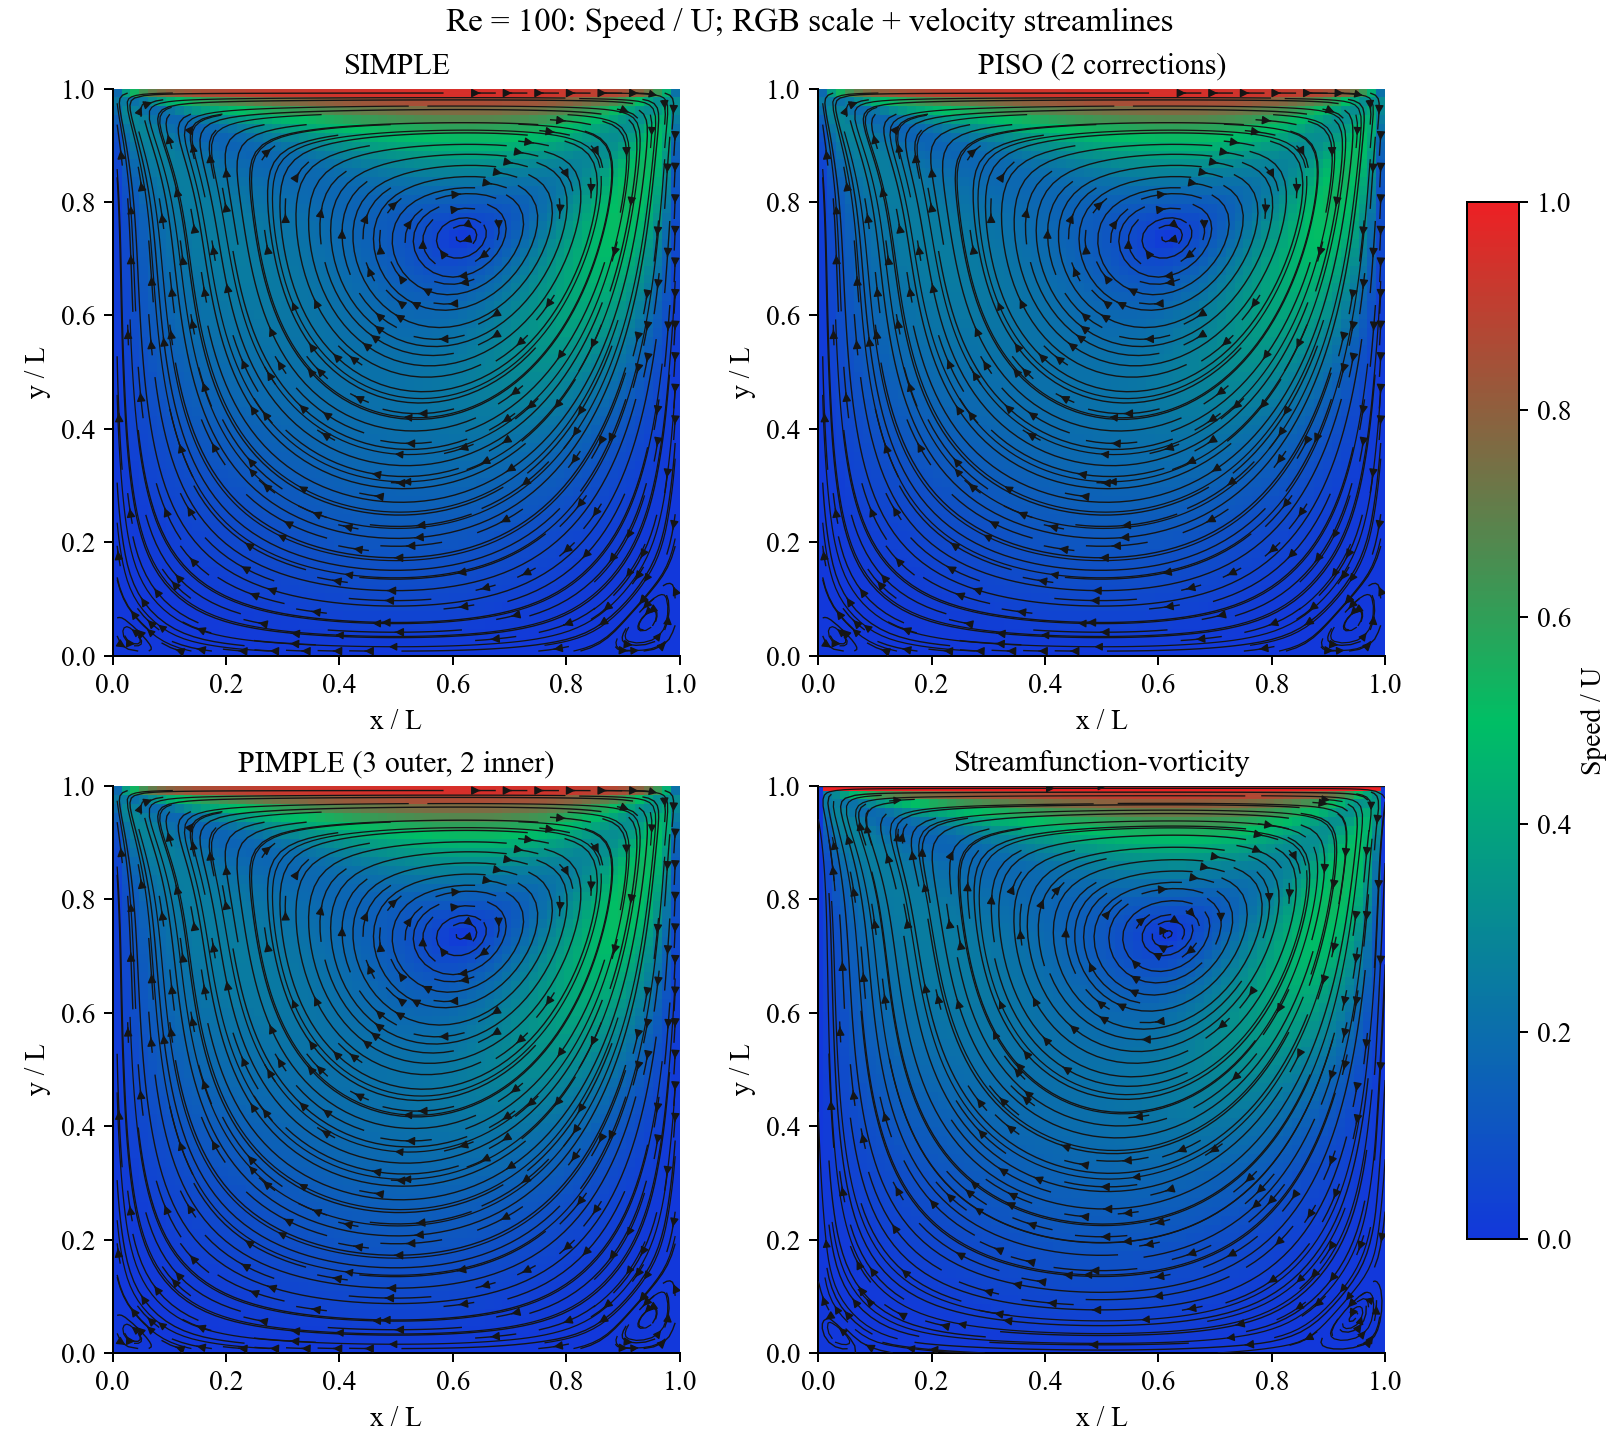
\includegraphics[width=.98\linewidth,height=85mm,keepaspectratio]{../../results/week01_2_pressure_velocity/figures/speed.png}\end{center}
Speed is $|\boldsymbol u|=\sqrt{u^2+v^2}$ and signed vorticity is $\omega=\partial v/\partial x-\partial u/\partial y$. The moving lid drives a clockwise primary circulation and a lower-cavity return flow. Black streamlines follow computed velocity; they are not vorticity contours. Small corner eddies depend on resolution and convergence as well as display density.
\begin{center}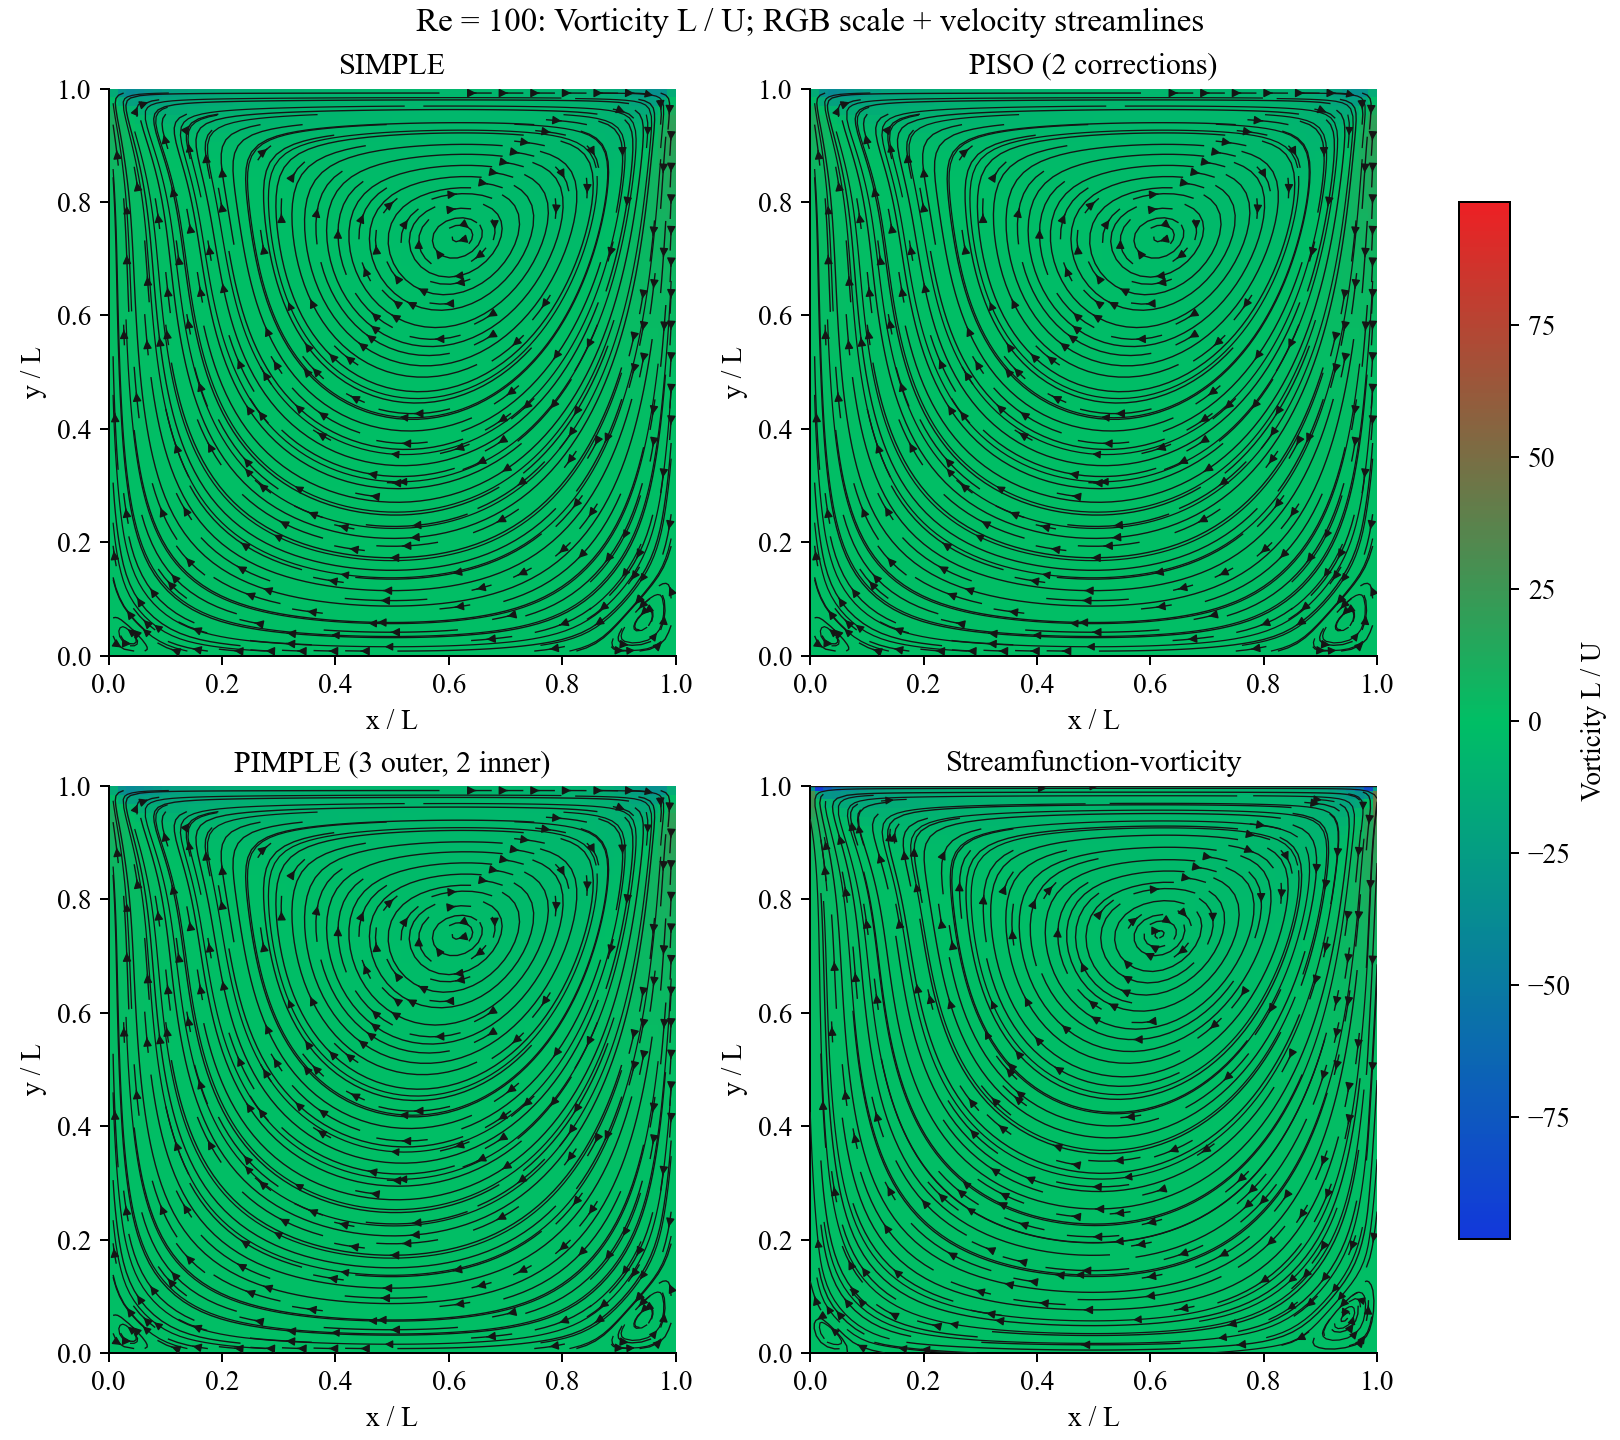
\includegraphics[width=.98\linewidth,height=85mm,keepaspectratio]{../../results/week01_2_pressure_velocity/figures/omega.png}\end{center}
Signed fields use a common symmetric-logarithmic color scale across methods, resolving interior values while retaining strong wall gradients. Colorbar values remain physical nondimensional field values. Similar converged fields are expected when the same discrete steady equations are solved; the comparison is useful for checking consistency.
\newpage
\topic{18}{Pressure and native convergence histories}
\begin{center}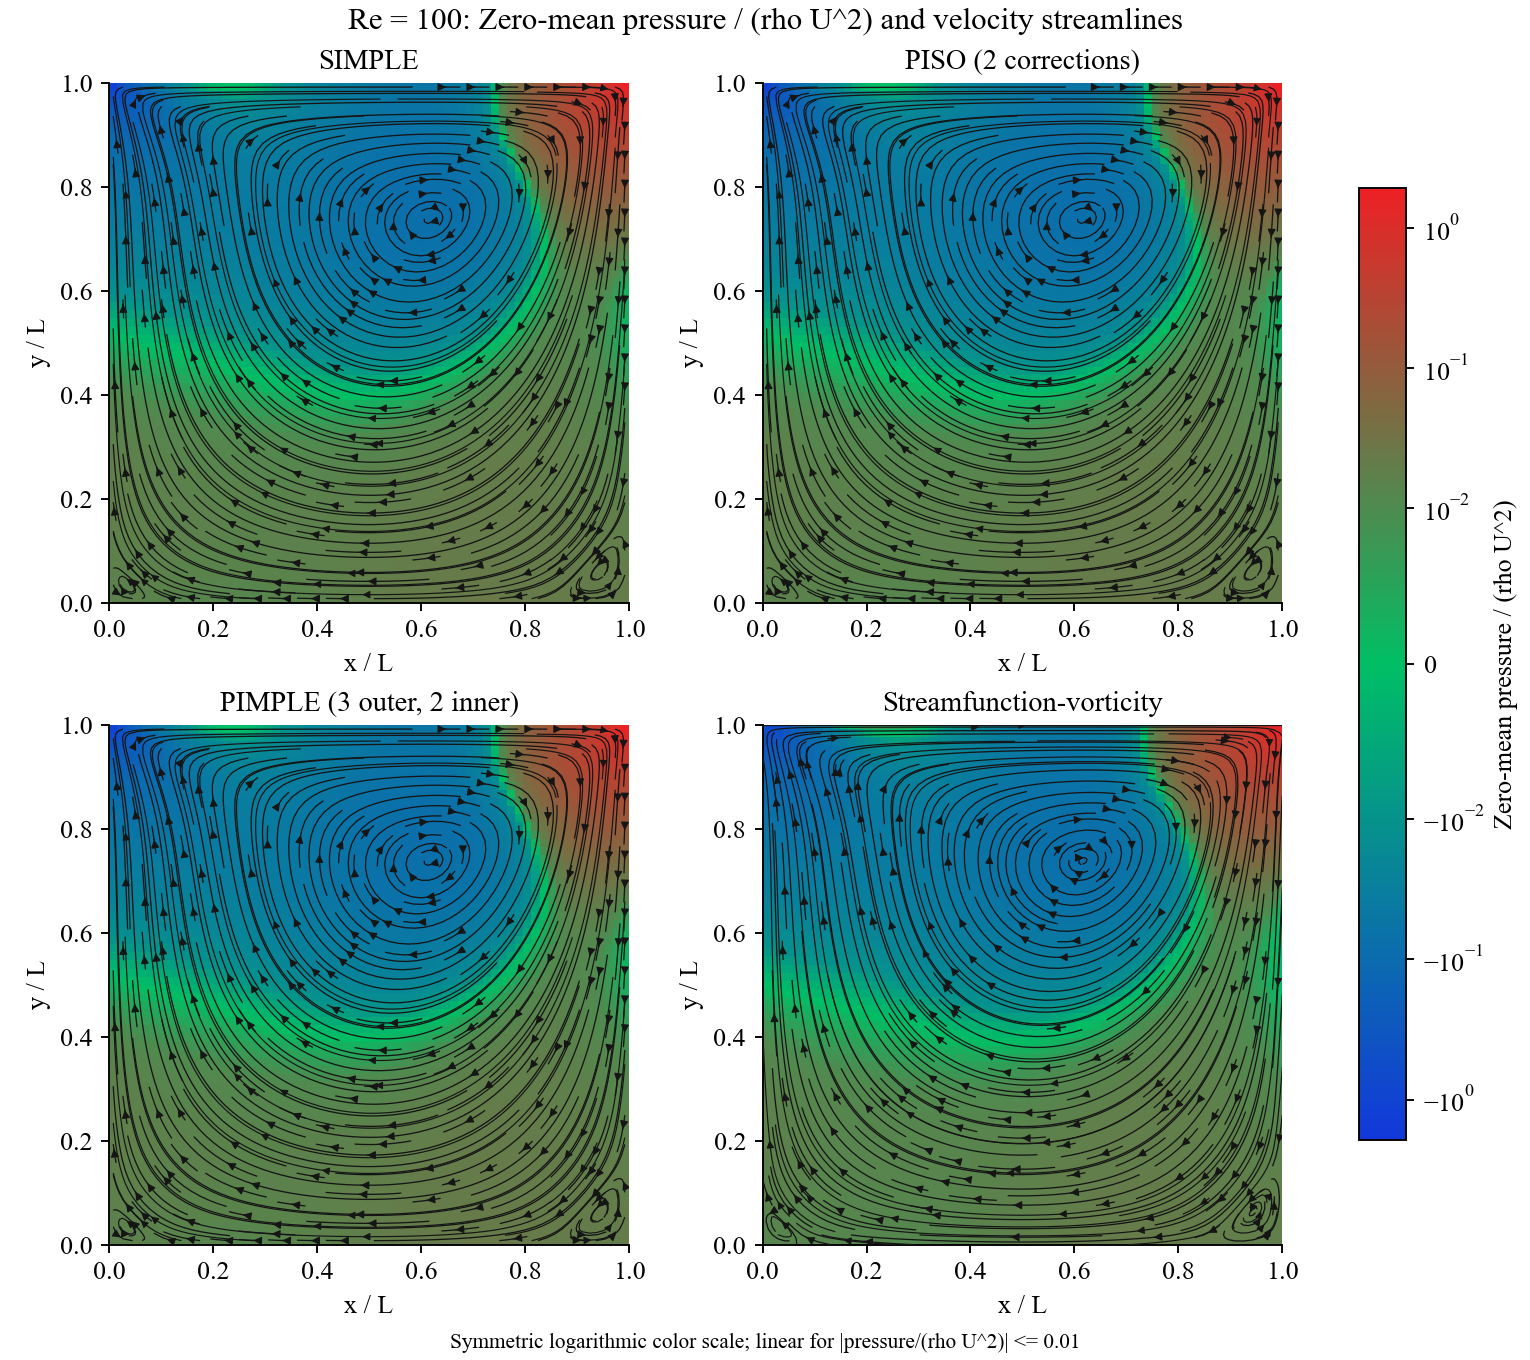
\includegraphics[width=.98\linewidth,height=89mm,keepaspectratio]{../../results/week01_2_pressure_velocity/figures/p.png}\end{center}
All pressures are reported with zero mean. Pressure gradients, rather than the arbitrary mean, affect velocity. Differences near the discontinuous lid corners should not be interpreted as reference-pressure validation. Ghia supplies velocity data, not pressure data.
\begin{center}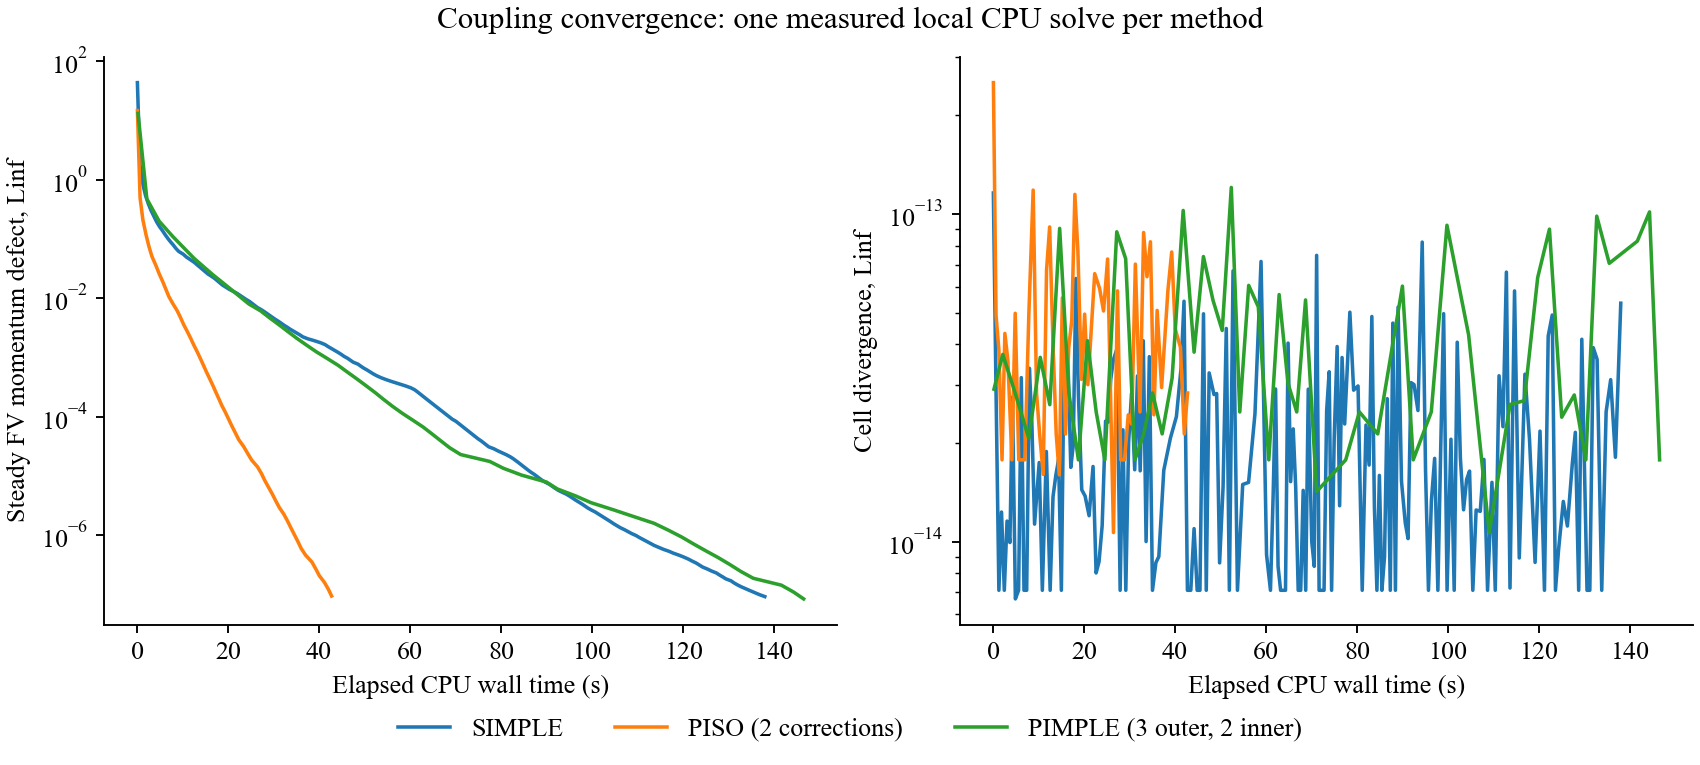
\includegraphics[width=.98\linewidth,height=70mm,keepaspectratio]{../../results/week01_2_pressure_velocity/figures/convergence.png}\end{center}
The finite-volume histories evaluate momentum and mass balance. The streamfunction solver's native vorticity-update norm is kept separate in the notebook because it is a different quantity. Timing comparisons still include that formulation. A small relaxed update alone is not a momentum-equation convergence test.
\newpage
\topic{19}{Accuracy and recorded cost at $Re=400$ and 1000}
\begin{center}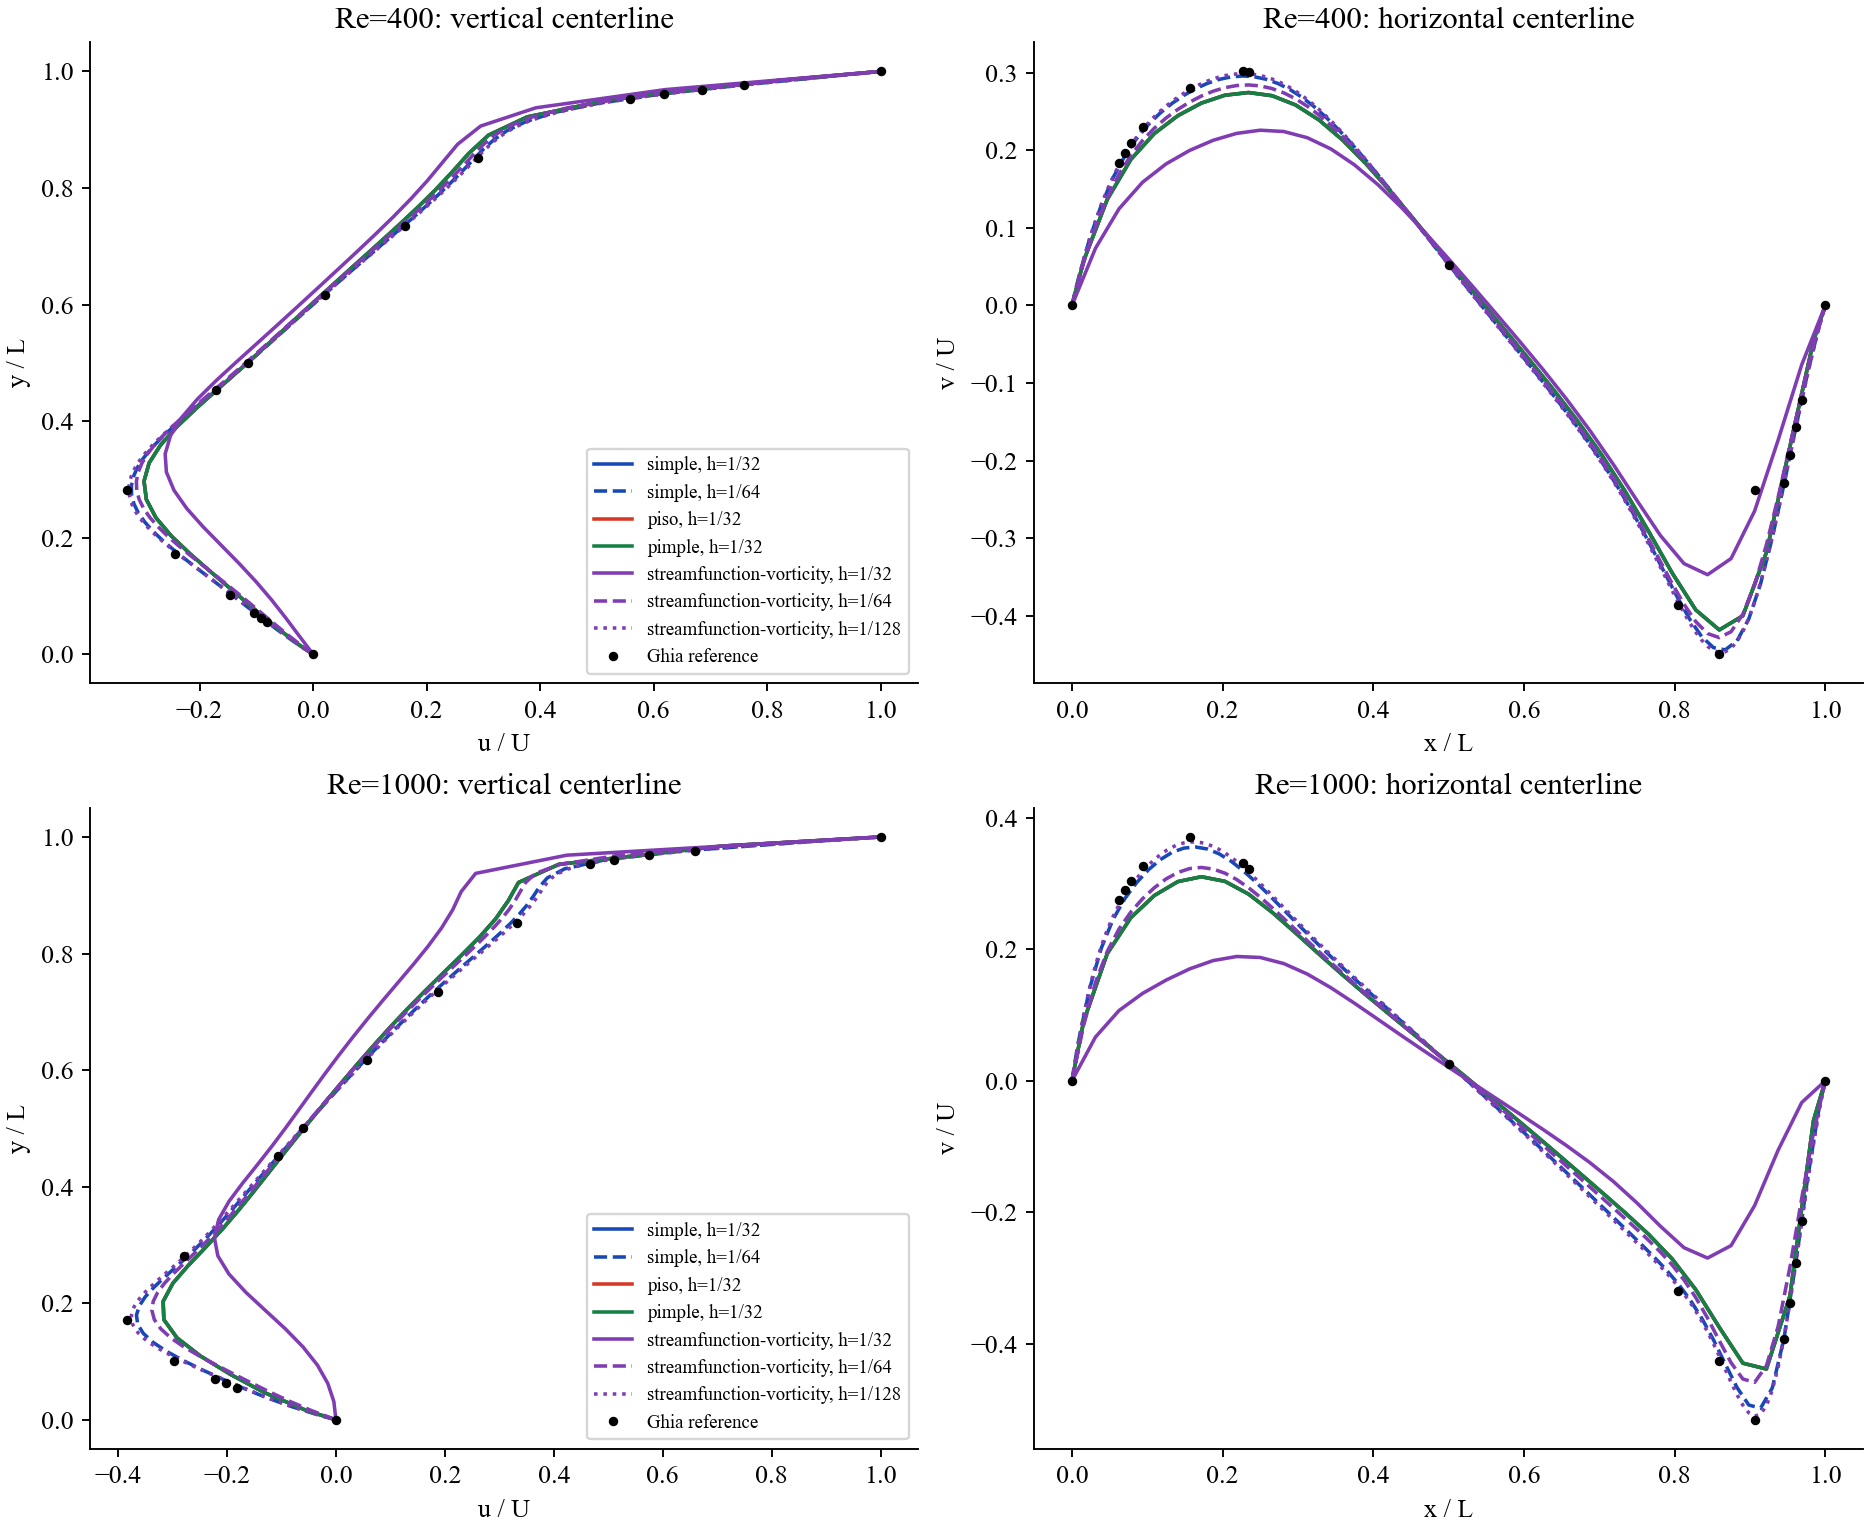
\includegraphics[width=.98\linewidth,height=94mm,keepaspectratio]{../../results/week01_2_formulations/centerlines.png}\end{center}
The retained study includes all four methods at $h=1/32$, plus selected finer meshes. A converged coarse-grid streamfunction result can have large reference error. At $Re=1000$, its 128-cell-spacing relative profile errors are approximately 2.0\% for $u$ and 1.7\% for $v$, using $\|f_{\rm computed}-f_{\rm Ghia}\|_2/\|f_{\rm Ghia}\|_2$ at the tabulated samples.
\begin{center}\small
\begin{tabular}{lrrr}\toprule
Formulation & $Re$ & Cells per side & Recorded seconds\\\midrule
PIMPLE & 400 & 32 & 96.949\\
PISO & 400 & 32 & 22.278\\
SIMPLE & 400 & 32 & 11.793\\
Streamfunction--vorticity & 400 & 32 & 78.475\\
SIMPLE & 400 & 64 & 71.061\\
Streamfunction--vorticity & 400 & 64 & 28.382\\
Streamfunction--vorticity & 400 & 128 & 70.928\\
PIMPLE & 1000 & 32 & 175.140\\
PISO & 1000 & 32 & 55.302\\
SIMPLE & 1000 & 32 & 12.459\\
Streamfunction--vorticity & 1000 & 32 & 175.065\\
SIMPLE & 1000 & 64 & 62.141\\
Streamfunction--vorticity & 1000 & 64 & 69.579\\
Streamfunction--vorticity & 1000 & 128 & 171.387\\
\bottomrule\end{tabular}\end{center}

For an error vector $z$ over the reference samples, $\|z\|_2=\sqrt{\sum_j z_j^2}$; $j$ labels a sampled location. These are recorded sequential local solver-call timings. Reference errors, mesh spacing and native stopping definitions accompany them. The $Re=400$ all-point $v$ error retains the isolated published entry; a separately labeled sensitivity metric omits that sample without replacing its value.
\newpage
\topic{20}{Mesh refinement and recirculation}
\begin{center}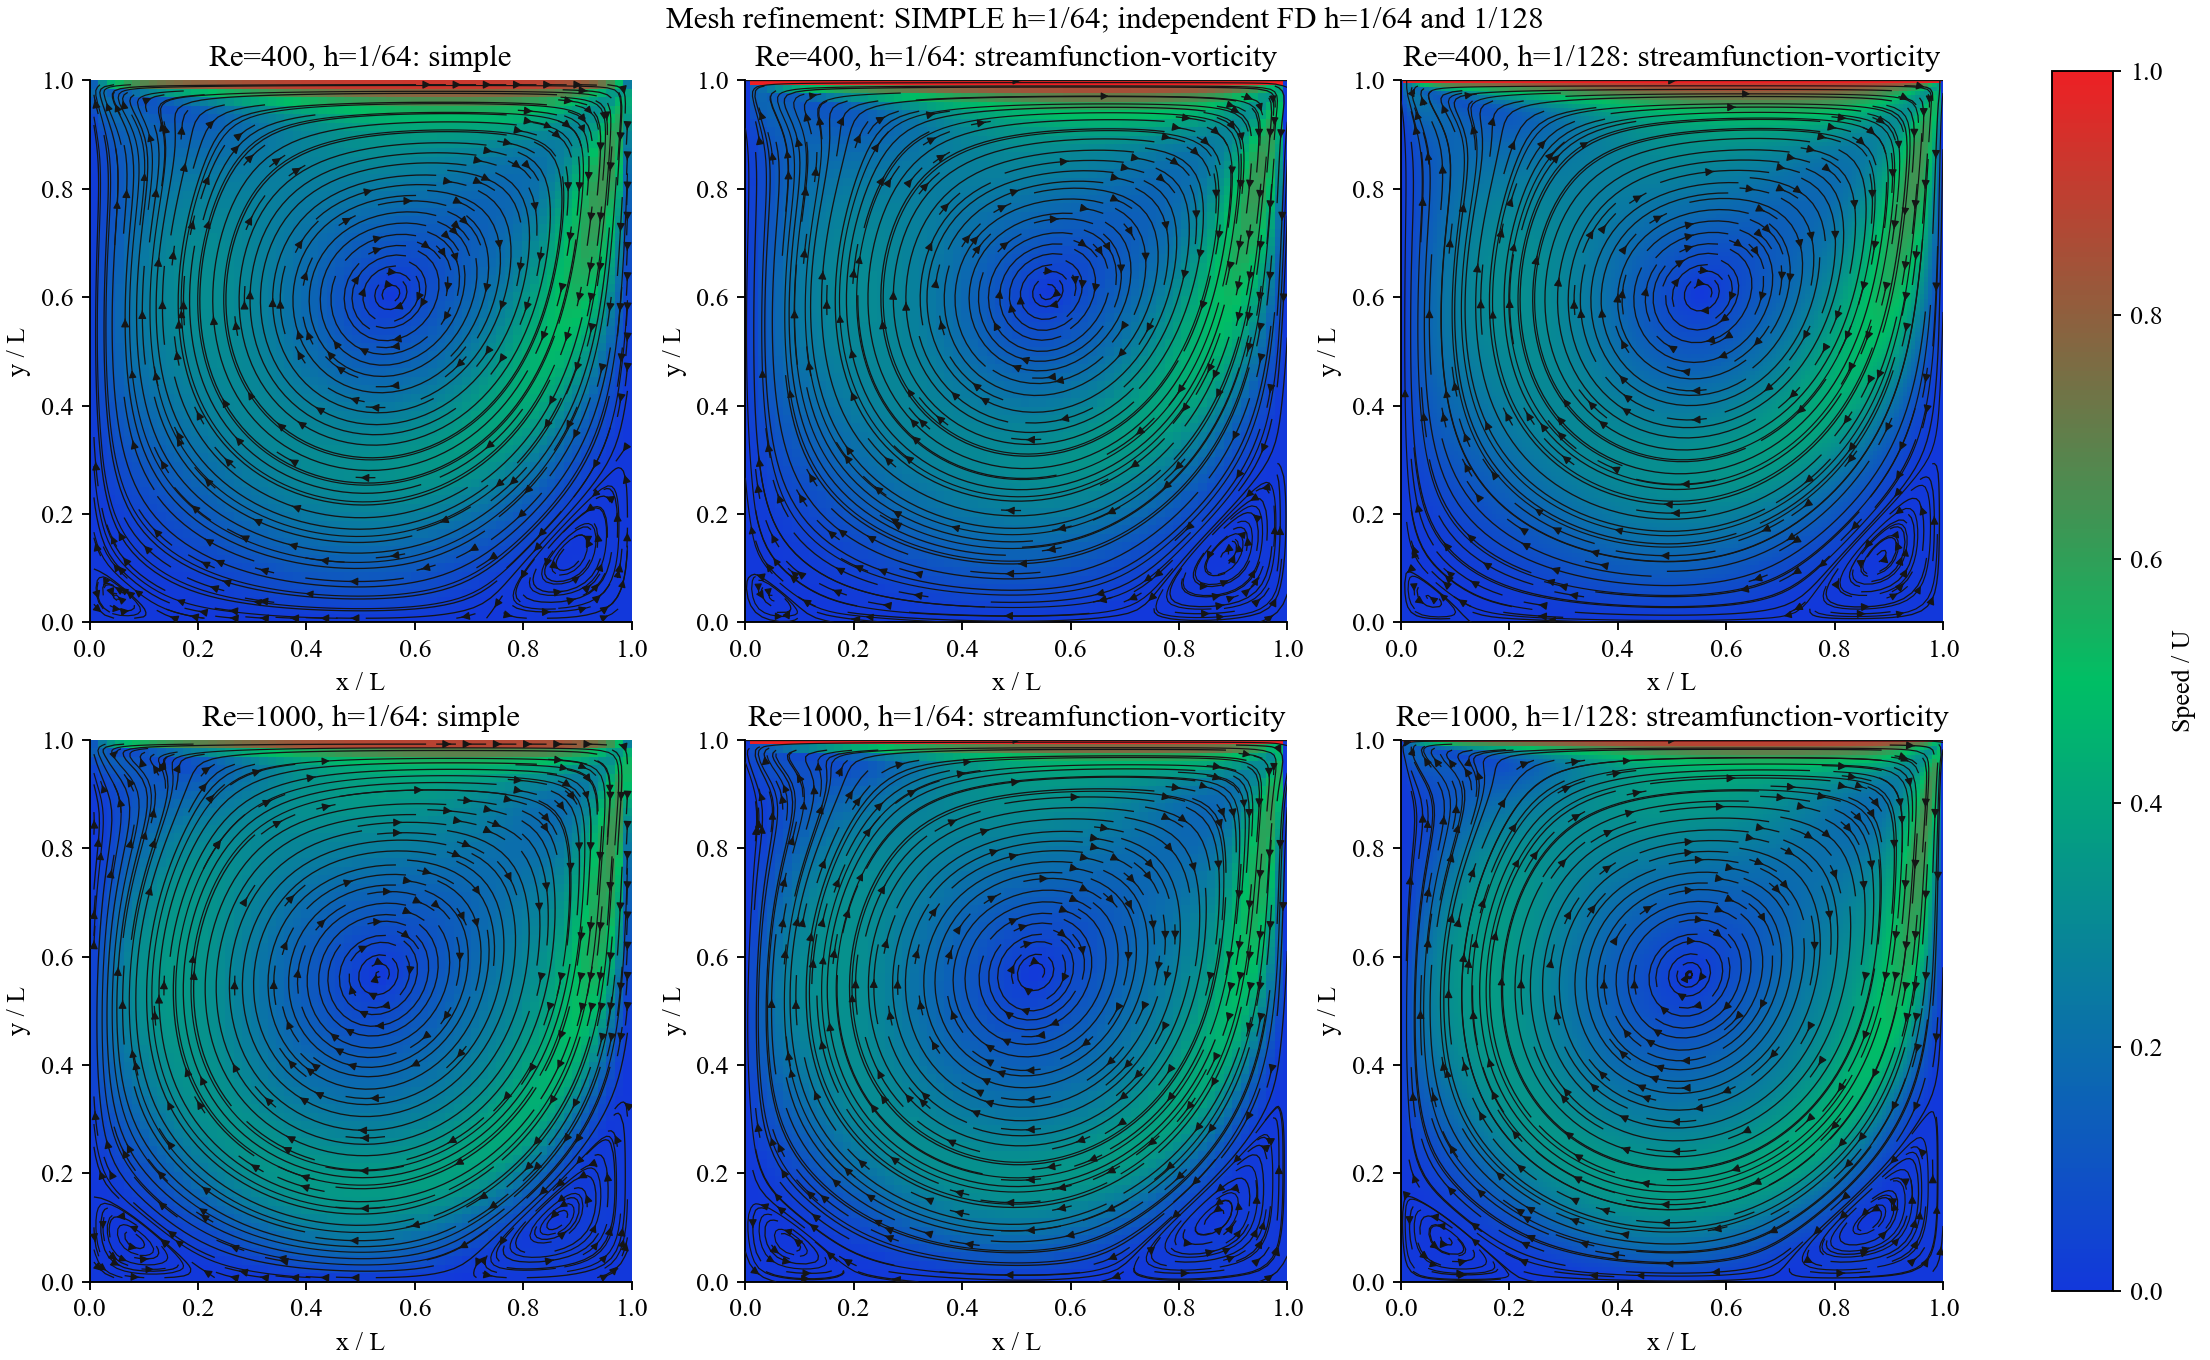
\includegraphics[width=.99\linewidth,height=150mm,keepaspectratio]{../../results/week01_2_formulations/refinement.png}\end{center}
Each panel states Reynolds number, formulation and spacing. The sampled primary-vortex location and resolved corner circulation change with refinement. More inner pressure corrections cannot reproduce an unresolved boundary layer or secondary vortex.

The fine-grid study is selected rather than a complete four-method refinement matrix. A result at one mesh does not demonstrate asymptotic order. Native steady-equation checks, Ghia errors and recorded initial failed attempts remain available with the data.

\textbf{Computational cost.} Fine grids and higher Reynolds numbers may require substantially longer runtimes and more memory. Students should begin with the supplied coarse case and estimate cost before selecting 64 or 128 cells on a laptop or Colab runtime.
\newpage
\topic{21}{A measured nonlinear coupling effect in the cavity}
\begin{center}\small
\begin{tabular}{lrrrrr}\toprule
Method & $\Delta t$ & Outer & Inner & Nonlinear momentum defect & Continuity defect\\\midrule
PISO & 0.01 & 1 & 1 & $1.61\times10^{0}$ & $5.90\times10^{-14}$\\
PISO & 0.01 & 1 & 2 & $1.78\times10^{-1}$ & $4.20\times10^{-14}$\\
PISO & 0.01 & 1 & 4 & $1.78\times10^{-1}$ & $4.26\times10^{-14}$\\
PIMPLE & 0.01 & 3 & 2 & $7.26\times10^{-6}$ & $5.23\times10^{-14}$\\
PIMPLE & 0.01 & 6 & 2 & $1.14\times10^{-12}$ & $6.84\times10^{-14}$\\
PISO & 0.05 & 1 & 1 & $5.13\times10^{0}$ & $7.27\times10^{-14}$\\
PISO & 0.05 & 1 & 2 & $1.11\times10^{0}$ & $2.38\times10^{-14}$\\
PISO & 0.05 & 1 & 4 & $1.12\times10^{0}$ & $2.96\times10^{-14}$\\
PIMPLE & 0.05 & 3 & 2 & $3.43\times10^{-3}$ & $4.92\times10^{-14}$\\
PIMPLE & 0.05 & 6 & 2 & $3.75\times10^{-7}$ & $4.93\times10^{-14}$\\
PISO & 0.2 & 1 & 1 & $9.34\times10^{0}$ & $1.37\times10^{-13}$\\
PISO & 0.2 & 1 & 2 & $2.39\times10^{0}$ & $8.88\times10^{-15}$\\
PISO & 0.2 & 1 & 4 & $2.47\times10^{0}$ & $1.14\times10^{-14}$\\
PIMPLE & 0.2 & 3 & 2 & $4.92\times10^{-2}$ & $9.77\times10^{-15}$\\
PIMPLE & 0.2 & 6 & 2 & $1.46\times10^{-4}$ & $3.38\times10^{-14}$\\
\bottomrule\end{tabular}\end{center}

Fifteen configurations start from rest at $Re=100$ on 32 cells per side. Each takes one backward-Euler step. At each fixed $\Delta t$, the study varies inner pressure corrections and outer coefficient updates.

The nonlinear step diagnostic rebuilds convection from the final velocity, while the frozen-predictor diagnostic uses the coefficients assembled for the predictor. Extra PISO corrections can reduce pressure--velocity inconsistency without eliminating the error from frozen nonlinear coefficients. PIMPLE also updates those coefficients, with additional momentum assembly and solves.

All retained cases in this one-step study satisfy a cell-divergence defect below $10^{-9}$. The remaining nonlinear momentum defects distinguish the correction strategies. Their differences demonstrate algebraic coupling behavior for this setup, not the accuracy of a transient trajectory.

Each panel has its own logarithmic vertical range. For a temporal-accuracy study, reduce $\Delta t$ and compare at matched physical times. More correctors and a stable larger time step do not establish an accurate startup history or a universal wall-time advantage.
\newpage
\topic{22}{Notebook controls and student analysis}
The notebook presents the same derivations and runnable algebraic examples, followed by retained CFD results. Fresh CFD runs are opt-in so the default lesson can be inspected without repeating every expensive calculation.
\begin{center}\begin{tabular}{ll}\toprule
Control & Purpose\\\midrule
\texttt{RUN\_NEW} & Fresh baseline calculation at $Re=100$\\
\texttt{RUN\_HIGHER\_RE} & Fresh experimental higher-$Re$ calculation\\
\texttt{HIGHER\_METHOD} & One method or all four formulations\\
\texttt{HIGHER\_CELLS} & Number of cells per side / matched FD spacing\\
\texttt{RUN\_STREAMFUNCTION} & Independent FD refinement experiment\\\bottomrule
\end{tabular}\end{center}
\textbf{Conservation.} Derive the four-face cell pressure equation and verify the two-cell example. Explain why a zero global flux does not guarantee zero cell imbalance. Add a constant pressure offset and check that velocities do not change.

\textbf{PISO.} Reproduce both corrections of the frozen-matrix example. Identify which quantities change between correctors. Explain why zero divergence after the first correction does not imply zero momentum defect.

\textbf{PIMPLE.} Reproduce the three outer passes of the nonlinear example. Evaluate the nonlinear defect using coefficients rebuilt from the final velocity. Explain why the old-time source must stay fixed. Compare one outer pass with PISO.

\textbf{Cavity comparison.} Start at $Re=100$ and matching mesh spacing. Record final cell divergence, unrelaxed momentum defect, both Ghia profile errors, runtime, and solve counts. Change one coupling setting at a time; keep spatial equations and final accuracy targets fixed.

\textbf{Higher Reynolds number.} At $Re=400$ and 1000, separate spatial refinement from coupling changes. Retain failed configurations. State the cost before proposing a fine-grid run. Native FD and FV residual magnitudes must not be interpreted as the same error.

\textbf{Transient extension.} Specify a final physical time, run a sequence of halved time steps, and compare common field or phase errors. Keep the time scheme fixed when comparing coupling algorithms. The current steady SIMPLE iteration is not a transient trajectory.
\newpage
\topic{23}{References}
The textbook treatments develop finite-volume conservation, staggered pressure--velocity coupling and pressure correction. The paper and official algorithm documentation provide the PISO origin and practical inner/outer-loop distinctions.
\begin{enumerate}[label={[\arabic*]}]
\item S. V. Patankar (1980). \emph{Numerical Heat Transfer and Fluid Flow}. Hemisphere/Taylor \& Francis. \href{https://www.routledge.com/Numerical-Heat-Transfer-and-Fluid-Flow/Patankar/p/book/9780891165224}{Publisher}. Foundational pressure correction, staggered grids and SIMPLE.
\item H. K. Versteeg and W. Malalasekera (2007). \emph{An Introduction to Computational Fluid Dynamics: The Finite Volume Method}, 2nd ed. Pearson. \href{https://www.pearson.com/en-gb/subject-catalog/p/Versteeg-An-Introduction-to-Computational-Fluid-Dynamics-The-Finite-Volume-Method-2nd-Edition/P200000005670?view=educator}{Publisher}. Finite-volume transport and pressure--velocity coupling.
\item J. H. Ferziger, M. Peri\'c and R. L. Street (2020). \emph{Computational Methods for Fluid Dynamics}, 4th ed. Springer. \href{https://doi.org/10.1007/978-3-319-99693-6}{doi:10.1007/978-3-319-99693-6}. Incompressible-flow solution methods and numerical errors.
\item F. Moukalled, L. Mangani and M. Darwish (2016). \emph{The Finite Volume Method in Computational Fluid Dynamics}. Chapter 15, ``Fluid Flow Computation: Incompressible Flows,'' pp. 561--654. \href{https://doi.org/10.1007/978-3-319-16874-6_15}{Chapter DOI}. Staggered/collocated arrangements and SIMPLE/PISO derivations.
\item R. I. Issa (1986). ``Solution of the implicitly discretised fluid flow equations by operator-splitting.'' \emph{Journal of Computational Physics} 62(1), 40--65. \href{https://doi.org/10.1016/0021-9991(86)90099-9}{doi:10.1016/0021-9991(86)90099-9}. Original PISO formulation.
\item CFD Direct, \emph{OpenFOAM User Guide v13}, sections 4.6.7--4.6.8. \href{https://doc.cfd.direct/openfoam/user-guide-v13/fvsolution}{Solution and algorithm control}. Pressure reference, correctors and outer correctors. The teaching solver's fixed-loop MAC implementation is specified in the preceding equations; software variants need not have identical defaults.
\item OpenCFD, \emph{Pressure--velocity coupling}. \href{https://doc.openfoam.com/2306/tools/processing/solvers/pressure-velocity/}{Official equation decomposition}. Momentum diagonal and neighbor-source representation.
\item U. Ghia, K. N. Ghia and C. T. Shin (1982). ``High-Re solutions for incompressible flow using the Navier--Stokes equations and a multigrid method.'' \emph{JCP} 48, 387--411. \href{https://doi.org/10.1016/0021-9991(82)90058-4}{doi:10.1016/0021-9991(82)90058-4}. Velocity benchmark samples.
\end{enumerate}
The examples use a staggered grid. Collocated-grid interpolation and Rhie--Chow stabilization are separate topics and are not implemented by this solver.
\end{document}
